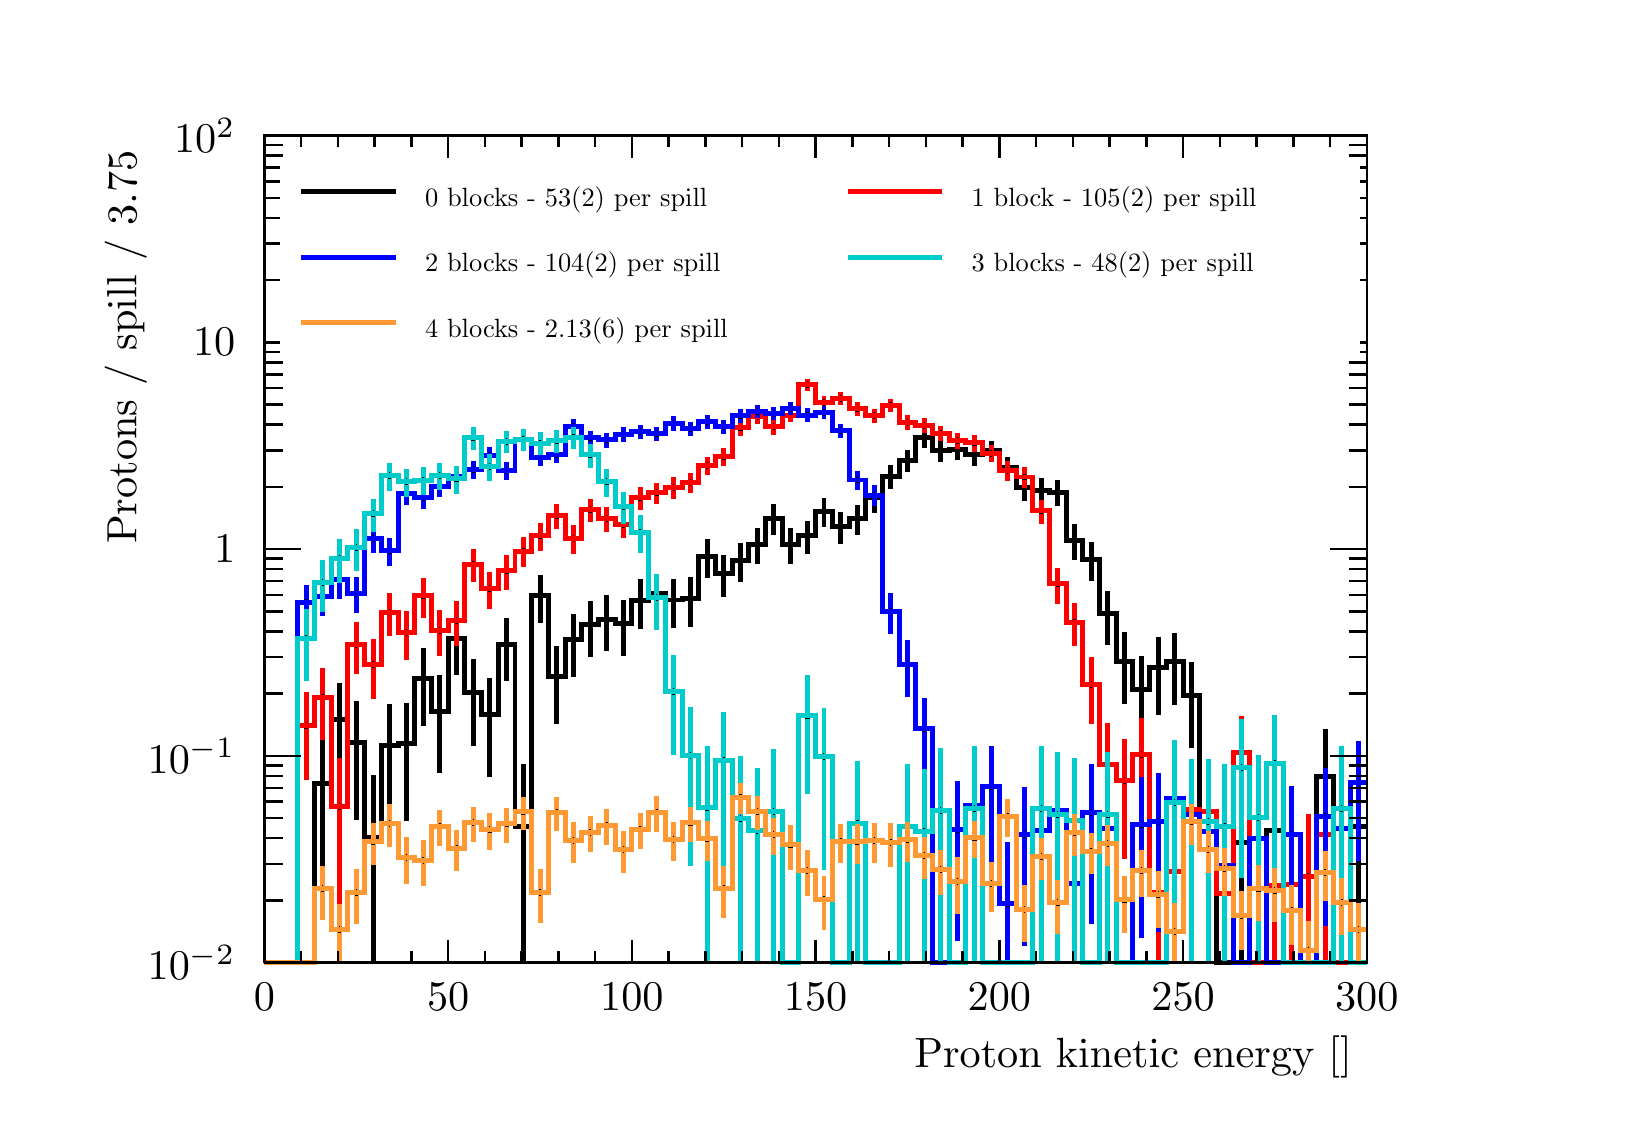
\begin{tikzpicture}
\pgfdeclareplotmark{cross} {
\pgfpathmoveto{\pgfpoint{-0.3\pgfplotmarksize}{\pgfplotmarksize}}
\pgfpathlineto{\pgfpoint{+0.3\pgfplotmarksize}{\pgfplotmarksize}}
\pgfpathlineto{\pgfpoint{+0.3\pgfplotmarksize}{0.3\pgfplotmarksize}}
\pgfpathlineto{\pgfpoint{+1\pgfplotmarksize}{0.3\pgfplotmarksize}}
\pgfpathlineto{\pgfpoint{+1\pgfplotmarksize}{-0.3\pgfplotmarksize}}
\pgfpathlineto{\pgfpoint{+0.3\pgfplotmarksize}{-0.3\pgfplotmarksize}}
\pgfpathlineto{\pgfpoint{+0.3\pgfplotmarksize}{-1.\pgfplotmarksize}}
\pgfpathlineto{\pgfpoint{-0.3\pgfplotmarksize}{-1.\pgfplotmarksize}}
\pgfpathlineto{\pgfpoint{-0.3\pgfplotmarksize}{-0.3\pgfplotmarksize}}
\pgfpathlineto{\pgfpoint{-1.\pgfplotmarksize}{-0.3\pgfplotmarksize}}
\pgfpathlineto{\pgfpoint{-1.\pgfplotmarksize}{0.3\pgfplotmarksize}}
\pgfpathlineto{\pgfpoint{-0.3\pgfplotmarksize}{0.3\pgfplotmarksize}}
\pgfpathclose
\pgfusepathqstroke
}
\pgfdeclareplotmark{cross*} {
\pgfpathmoveto{\pgfpoint{-0.3\pgfplotmarksize}{\pgfplotmarksize}}
\pgfpathlineto{\pgfpoint{+0.3\pgfplotmarksize}{\pgfplotmarksize}}
\pgfpathlineto{\pgfpoint{+0.3\pgfplotmarksize}{0.3\pgfplotmarksize}}
\pgfpathlineto{\pgfpoint{+1\pgfplotmarksize}{0.3\pgfplotmarksize}}
\pgfpathlineto{\pgfpoint{+1\pgfplotmarksize}{-0.3\pgfplotmarksize}}
\pgfpathlineto{\pgfpoint{+0.3\pgfplotmarksize}{-0.3\pgfplotmarksize}}
\pgfpathlineto{\pgfpoint{+0.3\pgfplotmarksize}{-1.\pgfplotmarksize}}
\pgfpathlineto{\pgfpoint{-0.3\pgfplotmarksize}{-1.\pgfplotmarksize}}
\pgfpathlineto{\pgfpoint{-0.3\pgfplotmarksize}{-0.3\pgfplotmarksize}}
\pgfpathlineto{\pgfpoint{-1.\pgfplotmarksize}{-0.3\pgfplotmarksize}}
\pgfpathlineto{\pgfpoint{-1.\pgfplotmarksize}{0.3\pgfplotmarksize}}
\pgfpathlineto{\pgfpoint{-0.3\pgfplotmarksize}{0.3\pgfplotmarksize}}
\pgfpathclose
\pgfusepathqfillstroke
}
\pgfdeclareplotmark{newstar} {
\pgfpathmoveto{\pgfqpoint{0pt}{\pgfplotmarksize}}
\pgfpathlineto{\pgfqpointpolar{44}{0.5\pgfplotmarksize}}
\pgfpathlineto{\pgfqpointpolar{18}{\pgfplotmarksize}}
\pgfpathlineto{\pgfqpointpolar{-20}{0.5\pgfplotmarksize}}
\pgfpathlineto{\pgfqpointpolar{-54}{\pgfplotmarksize}}
\pgfpathlineto{\pgfqpointpolar{-90}{0.5\pgfplotmarksize}}
\pgfpathlineto{\pgfqpointpolar{234}{\pgfplotmarksize}}
\pgfpathlineto{\pgfqpointpolar{198}{0.5\pgfplotmarksize}}
\pgfpathlineto{\pgfqpointpolar{162}{\pgfplotmarksize}}
\pgfpathlineto{\pgfqpointpolar{134}{0.5\pgfplotmarksize}}
\pgfpathclose
\pgfusepathqstroke
}
\pgfdeclareplotmark{newstar*} {
\pgfpathmoveto{\pgfqpoint{0pt}{\pgfplotmarksize}}
\pgfpathlineto{\pgfqpointpolar{44}{0.5\pgfplotmarksize}}
\pgfpathlineto{\pgfqpointpolar{18}{\pgfplotmarksize}}
\pgfpathlineto{\pgfqpointpolar{-20}{0.5\pgfplotmarksize}}
\pgfpathlineto{\pgfqpointpolar{-54}{\pgfplotmarksize}}
\pgfpathlineto{\pgfqpointpolar{-90}{0.5\pgfplotmarksize}}
\pgfpathlineto{\pgfqpointpolar{234}{\pgfplotmarksize}}
\pgfpathlineto{\pgfqpointpolar{198}{0.5\pgfplotmarksize}}
\pgfpathlineto{\pgfqpointpolar{162}{\pgfplotmarksize}}
\pgfpathlineto{\pgfqpointpolar{134}{0.5\pgfplotmarksize}}
\pgfpathclose
\pgfusepathqfillstroke
}
\definecolor{c}{rgb}{1,1,1};
\draw [color=c, fill=c] (0,0) rectangle (20,13.639);
\draw [color=c, fill=c] (3,1.77307) rectangle (17,12.2751);
\definecolor{c}{rgb}{0,0,0};
\draw [c,line width=0.9] (3,1.77307) -- (3,12.2751) -- (17,12.2751) -- (17,1.77307) -- (3,1.77307);
\definecolor{c}{rgb}{1,1,1};
\draw [color=c, fill=c] (3,1.77307) rectangle (17,12.2751);
\definecolor{c}{rgb}{0,0,0};
\draw [c,line width=0.9] (3,1.77307) -- (3,12.2751) -- (17,12.2751) -- (17,1.77307) -- (3,1.77307);
\draw [c,line width=0.9] (3,1.77307) -- (3.21212,1.77307) -- (3.21212,1.77307) -- (3.42424,1.77307) -- (3.42424,1.77307) -- (3.63636,1.77307) -- (3.63636,1.77307) -- (3.84848,1.77307) -- (3.84848,1.77307) -- (4.06061,1.77307) -- (4.06061,1.77307) --
 (4.27273,1.77307) -- (4.27273,1.77307) -- (4.48485,1.77307) -- (4.48485,1.77307) -- (4.69697,1.77307) -- (4.69697,1.77307) -- (4.90909,1.77307) -- (4.90909,1.77307) -- (5.12121,1.77307) -- (5.12121,1.77307) -- (5.33333,1.77307) -- (5.33333,1.77307)
 -- (5.54545,1.77307) -- (5.54545,1.77307) -- (5.75758,1.77307) -- (5.75758,1.77307) -- (5.9697,1.77307) -- (5.9697,1.77307) -- (6.18182,1.77307) -- (6.18182,1.77307) -- (6.39394,1.77307) -- (6.39394,1.77307) -- (6.60606,1.77307) -- (6.60606,1.77307)
 -- (6.81818,1.77307) -- (6.81818,1.77307) -- (7.0303,1.77307) -- (7.0303,1.77307) -- (7.24242,1.77307) -- (7.24242,1.77307) -- (7.45455,1.77307) -- (7.45455,1.77307) -- (7.66667,1.77307) -- (7.66667,1.77307) -- (7.87879,1.77307) -- (7.87879,1.77307)
 -- (8.09091,1.77307) -- (8.09091,1.77307) -- (8.30303,1.77307) -- (8.30303,1.77307) -- (8.51515,1.77307) -- (8.51515,1.77307) -- (8.72727,1.77307) -- (8.72727,1.77307) -- (8.93939,1.77307) -- (8.93939,1.77307) -- (9.15152,1.77307) --
 (9.15152,1.77307) -- (9.36364,1.77307) -- (9.36364,1.77307) -- (9.57576,1.77307) -- (9.57576,1.77307) -- (9.78788,1.77307) -- (9.78788,1.77307) -- (10,1.77307) -- (10,1.77307) -- (10.2121,1.77307) -- (10.2121,1.77307) -- (10.4242,1.77307) --
 (10.4242,1.77307) -- (10.6364,1.77307) -- (10.6364,1.77307) -- (10.8485,1.77307) -- (10.8485,1.77307) -- (11.0606,1.77307) -- (11.0606,1.77307) -- (11.2727,1.77307) -- (11.2727,1.77307) -- (11.4848,1.77307) -- (11.4848,1.77307) -- (11.697,1.77307)
 -- (11.697,1.77307) -- (11.9091,1.77307) -- (11.9091,1.77307) -- (12.1212,1.77307) -- (12.1212,1.77307) -- (12.3333,1.77307) -- (12.3333,1.77307) -- (12.5455,1.77307) -- (12.5455,1.77307) -- (12.7576,1.77307) -- (12.7576,1.77307) --
 (12.9697,1.77307) -- (12.9697,1.77307) -- (13.1818,1.77307) -- (13.1818,1.77307) -- (13.3939,1.77307) -- (13.3939,1.77307) -- (13.6061,1.77307) -- (13.6061,1.77307) -- (13.8182,1.77307) -- (13.8182,1.77307) -- (14.0303,1.77307) -- (14.0303,1.77307)
 -- (14.2424,1.77307) -- (14.2424,1.77307) -- (14.4545,1.77307) -- (14.4545,1.77307) -- (14.6667,1.77307) -- (14.6667,1.77307) -- (14.8788,1.77307) -- (14.8788,1.77307) -- (15.0909,1.77307) -- (15.0909,1.77307) -- (15.303,1.77307) -- (15.303,1.77307)
 -- (15.5152,1.77307) -- (15.5152,1.77307) -- (15.7273,1.77307) -- (15.7273,1.77307) -- (15.9394,1.77307) -- (15.9394,1.77307) -- (16.1515,1.77307) -- (16.1515,1.77307) -- (16.3636,1.77307) -- (16.3636,1.77307) -- (16.5758,1.77307) --
 (16.5758,1.77307) -- (16.7879,1.77307) -- (16.7879,1.77307) -- (17,1.77307);
\draw [c,line width=0.9] (3,1.77307) -- (17,1.77307);
\draw [c,line width=0.9] (3,2.05948) -- (3,1.77307);
\draw [c,line width=0.9] (3.46667,1.91628) -- (3.46667,1.77307);
\draw [c,line width=0.9] (3.93333,1.91628) -- (3.93333,1.77307);
\draw [c,line width=0.9] (4.4,1.91628) -- (4.4,1.77307);
\draw [c,line width=0.9] (4.86667,1.91628) -- (4.86667,1.77307);
\draw [c,line width=0.9] (5.33333,2.05948) -- (5.33333,1.77307);
\draw [c,line width=0.9] (5.8,1.91628) -- (5.8,1.77307);
\draw [c,line width=0.9] (6.26667,1.91628) -- (6.26667,1.77307);
\draw [c,line width=0.9] (6.73333,1.91628) -- (6.73333,1.77307);
\draw [c,line width=0.9] (7.2,1.91628) -- (7.2,1.77307);
\draw [c,line width=0.9] (7.66667,2.05948) -- (7.66667,1.77307);
\draw [c,line width=0.9] (8.13333,1.91628) -- (8.13333,1.77307);
\draw [c,line width=0.9] (8.6,1.91628) -- (8.6,1.77307);
\draw [c,line width=0.9] (9.06667,1.91628) -- (9.06667,1.77307);
\draw [c,line width=0.9] (9.53333,1.91628) -- (9.53333,1.77307);
\draw [c,line width=0.9] (10,2.05948) -- (10,1.77307);
\draw [c,line width=0.9] (10.4667,1.91628) -- (10.4667,1.77307);
\draw [c,line width=0.9] (10.9333,1.91628) -- (10.9333,1.77307);
\draw [c,line width=0.9] (11.4,1.91628) -- (11.4,1.77307);
\draw [c,line width=0.9] (11.8667,1.91628) -- (11.8667,1.77307);
\draw [c,line width=0.9] (12.3333,2.05948) -- (12.3333,1.77307);
\draw [c,line width=0.9] (12.8,1.91628) -- (12.8,1.77307);
\draw [c,line width=0.9] (13.2667,1.91628) -- (13.2667,1.77307);
\draw [c,line width=0.9] (13.7333,1.91628) -- (13.7333,1.77307);
\draw [c,line width=0.9] (14.2,1.91628) -- (14.2,1.77307);
\draw [c,line width=0.9] (14.6667,2.05948) -- (14.6667,1.77307);
\draw [c,line width=0.9] (15.1333,1.91628) -- (15.1333,1.77307);
\draw [c,line width=0.9] (15.6,1.91628) -- (15.6,1.77307);
\draw [c,line width=0.9] (16.0667,1.91628) -- (16.0667,1.77307);
\draw [c,line width=0.9] (16.5333,1.91628) -- (16.5333,1.77307);
\draw [c,line width=0.9] (17,2.05948) -- (17,1.77307);
\draw [c,line width=0.9] (17,2.05948) -- (17,1.77307);
\draw [anchor=base] (3,1.15931) node[scale=1.52731, color=c, rotate=0]{0};
\draw [anchor=base] (5.33333,1.15931) node[scale=1.52731, color=c, rotate=0]{50};
\draw [anchor=base] (7.66667,1.15931) node[scale=1.52731, color=c, rotate=0]{100};
\draw [anchor=base] (10,1.15931) node[scale=1.52731, color=c, rotate=0]{150};
\draw [anchor=base] (12.3333,1.15931) node[scale=1.52731, color=c, rotate=0]{200};
\draw [anchor=base] (14.6667,1.15931) node[scale=1.52731, color=c, rotate=0]{250};
\draw [anchor=base] (17,1.15931) node[scale=1.52731, color=c, rotate=0]{300};
\draw [anchor= east] (17,0.572837) node[scale=1.52731, color=c, rotate=0]{ Proton kinetic energy [\si{\mega\electronvolt}] };
\draw [c,line width=0.9] (3,12.2751) -- (17,12.2751);
\draw [c,line width=0.9] (3,11.9887) -- (3,12.2751);
\draw [c,line width=0.9] (3.46667,12.1319) -- (3.46667,12.2751);
\draw [c,line width=0.9] (3.93333,12.1319) -- (3.93333,12.2751);
\draw [c,line width=0.9] (4.4,12.1319) -- (4.4,12.2751);
\draw [c,line width=0.9] (4.86667,12.1319) -- (4.86667,12.2751);
\draw [c,line width=0.9] (5.33333,11.9887) -- (5.33333,12.2751);
\draw [c,line width=0.9] (5.8,12.1319) -- (5.8,12.2751);
\draw [c,line width=0.9] (6.26667,12.1319) -- (6.26667,12.2751);
\draw [c,line width=0.9] (6.73333,12.1319) -- (6.73333,12.2751);
\draw [c,line width=0.9] (7.2,12.1319) -- (7.2,12.2751);
\draw [c,line width=0.9] (7.66667,11.9887) -- (7.66667,12.2751);
\draw [c,line width=0.9] (8.13333,12.1319) -- (8.13333,12.2751);
\draw [c,line width=0.9] (8.6,12.1319) -- (8.6,12.2751);
\draw [c,line width=0.9] (9.06667,12.1319) -- (9.06667,12.2751);
\draw [c,line width=0.9] (9.53333,12.1319) -- (9.53333,12.2751);
\draw [c,line width=0.9] (10,11.9887) -- (10,12.2751);
\draw [c,line width=0.9] (10.4667,12.1319) -- (10.4667,12.2751);
\draw [c,line width=0.9] (10.9333,12.1319) -- (10.9333,12.2751);
\draw [c,line width=0.9] (11.4,12.1319) -- (11.4,12.2751);
\draw [c,line width=0.9] (11.8667,12.1319) -- (11.8667,12.2751);
\draw [c,line width=0.9] (12.3333,11.9887) -- (12.3333,12.2751);
\draw [c,line width=0.9] (12.8,12.1319) -- (12.8,12.2751);
\draw [c,line width=0.9] (13.2667,12.1319) -- (13.2667,12.2751);
\draw [c,line width=0.9] (13.7333,12.1319) -- (13.7333,12.2751);
\draw [c,line width=0.9] (14.2,12.1319) -- (14.2,12.2751);
\draw [c,line width=0.9] (14.6667,11.9887) -- (14.6667,12.2751);
\draw [c,line width=0.9] (15.1333,12.1319) -- (15.1333,12.2751);
\draw [c,line width=0.9] (15.6,12.1319) -- (15.6,12.2751);
\draw [c,line width=0.9] (16.0667,12.1319) -- (16.0667,12.2751);
\draw [c,line width=0.9] (16.5333,12.1319) -- (16.5333,12.2751);
\draw [c,line width=0.9] (17,11.9887) -- (17,12.2751);
\draw [c,line width=0.9] (17,11.9887) -- (17,12.2751);
\draw [c,line width=0.9] (3,1.77307) -- (3,12.2751);
\draw [c,line width=0.9] (3.462,1.77307) -- (3,1.77307);
\draw [anchor= east] (2.82,1.77307) node[scale=1.52731, color=c, rotate=0]{$10^{-2}$};
\draw [c,line width=0.9] (3.231,2.56342) -- (3,2.56342);
\draw [c,line width=0.9] (3.231,3.02575) -- (3,3.02575);
\draw [c,line width=0.9] (3.231,3.35378) -- (3,3.35378);
\draw [c,line width=0.9] (3.231,3.60821) -- (3,3.60821);
\draw [c,line width=0.9] (3.231,3.81611) -- (3,3.81611);
\draw [c,line width=0.9] (3.231,3.99187) -- (3,3.99187);
\draw [c,line width=0.9] (3.231,4.14413) -- (3,4.14413);
\draw [c,line width=0.9] (3.231,4.27843) -- (3,4.27843);
\draw [c,line width=0.9] (3.462,4.39857) -- (3,4.39857);
\draw [anchor= east] (2.82,4.39857) node[scale=1.52731, color=c, rotate=0]{$10^{-1}$};
\draw [c,line width=0.9] (3.231,5.18892) -- (3,5.18892);
\draw [c,line width=0.9] (3.231,5.65125) -- (3,5.65125);
\draw [c,line width=0.9] (3.231,5.97928) -- (3,5.97928);
\draw [c,line width=0.9] (3.231,6.23372) -- (3,6.23372);
\draw [c,line width=0.9] (3.231,6.44161) -- (3,6.44161);
\draw [c,line width=0.9] (3.231,6.61737) -- (3,6.61737);
\draw [c,line width=0.9] (3.231,6.76963) -- (3,6.76963);
\draw [c,line width=0.9] (3.231,6.90393) -- (3,6.90393);
\draw [c,line width=0.9] (3.462,7.02407) -- (3,7.02407);
\draw [anchor= east] (2.82,7.02407) node[scale=1.52731, color=c, rotate=0]{1};
\draw [c,line width=0.9] (3.231,7.81442) -- (3,7.81442);
\draw [c,line width=0.9] (3.231,8.27675) -- (3,8.27675);
\draw [c,line width=0.9] (3.231,8.60478) -- (3,8.60478);
\draw [c,line width=0.9] (3.231,8.85922) -- (3,8.85922);
\draw [c,line width=0.9] (3.231,9.06711) -- (3,9.06711);
\draw [c,line width=0.9] (3.231,9.24288) -- (3,9.24288);
\draw [c,line width=0.9] (3.231,9.39513) -- (3,9.39513);
\draw [c,line width=0.9] (3.231,9.52943) -- (3,9.52943);
\draw [c,line width=0.9] (3.462,9.64957) -- (3,9.64957);
\draw [anchor= east] (2.82,9.64957) node[scale=1.52731, color=c, rotate=0]{10};
\draw [c,line width=0.9] (3.231,10.4399) -- (3,10.4399);
\draw [c,line width=0.9] (3.231,10.9023) -- (3,10.9023);
\draw [c,line width=0.9] (3.231,11.2303) -- (3,11.2303);
\draw [c,line width=0.9] (3.231,11.4847) -- (3,11.4847);
\draw [c,line width=0.9] (3.231,11.6926) -- (3,11.6926);
\draw [c,line width=0.9] (3.231,11.8684) -- (3,11.8684);
\draw [c,line width=0.9] (3.231,12.0206) -- (3,12.0206);
\draw [c,line width=0.9] (3.231,12.1549) -- (3,12.1549);
\draw [c,line width=0.9] (3.462,12.2751) -- (3,12.2751);
\draw [anchor= east] (2.82,12.2751) node[scale=1.52731, color=c, rotate=0]{$10^{2}$};
\draw [anchor= east] (1.24,12.2751) node[scale=1.52731, color=c, rotate=90]{ Protons / spill / \SI{3.75}{\mega\electronvolt} };
\draw [c,line width=0.9] (17,1.77307) -- (17,12.2751);
\draw [c,line width=0.9] (16.538,1.77307) -- (17,1.77307);
\draw [c,line width=0.9] (16.769,2.56342) -- (17,2.56342);
\draw [c,line width=0.9] (16.769,3.02575) -- (17,3.02575);
\draw [c,line width=0.9] (16.769,3.35378) -- (17,3.35378);
\draw [c,line width=0.9] (16.769,3.60821) -- (17,3.60821);
\draw [c,line width=0.9] (16.769,3.81611) -- (17,3.81611);
\draw [c,line width=0.9] (16.769,3.99187) -- (17,3.99187);
\draw [c,line width=0.9] (16.769,4.14413) -- (17,4.14413);
\draw [c,line width=0.9] (16.769,4.27843) -- (17,4.27843);
\draw [c,line width=0.9] (16.538,4.39857) -- (17,4.39857);
\draw [c,line width=0.9] (16.769,5.18892) -- (17,5.18892);
\draw [c,line width=0.9] (16.769,5.65125) -- (17,5.65125);
\draw [c,line width=0.9] (16.769,5.97928) -- (17,5.97928);
\draw [c,line width=0.9] (16.769,6.23372) -- (17,6.23372);
\draw [c,line width=0.9] (16.769,6.44161) -- (17,6.44161);
\draw [c,line width=0.9] (16.769,6.61737) -- (17,6.61737);
\draw [c,line width=0.9] (16.769,6.76963) -- (17,6.76963);
\draw [c,line width=0.9] (16.769,6.90393) -- (17,6.90393);
\draw [c,line width=0.9] (16.538,7.02407) -- (17,7.02407);
\draw [c,line width=0.9] (16.769,7.81442) -- (17,7.81442);
\draw [c,line width=0.9] (16.769,8.27675) -- (17,8.27675);
\draw [c,line width=0.9] (16.769,8.60478) -- (17,8.60478);
\draw [c,line width=0.9] (16.769,8.85922) -- (17,8.85922);
\draw [c,line width=0.9] (16.769,9.06711) -- (17,9.06711);
\draw [c,line width=0.9] (16.769,9.24288) -- (17,9.24288);
\draw [c,line width=0.9] (16.769,9.39513) -- (17,9.39513);
\draw [c,line width=0.9] (16.769,9.52943) -- (17,9.52943);
\draw [c,line width=0.9] (16.538,9.64957) -- (17,9.64957);
\draw [c,line width=0.9] (16.769,10.4399) -- (17,10.4399);
\draw [c,line width=0.9] (16.769,10.9023) -- (17,10.9023);
\draw [c,line width=0.9] (16.769,11.2303) -- (17,11.2303);
\draw [c,line width=0.9] (16.769,11.4847) -- (17,11.4847);
\draw [c,line width=0.9] (16.769,11.6926) -- (17,11.6926);
\draw [c,line width=0.9] (16.769,11.8684) -- (17,11.8684);
\draw [c,line width=0.9] (16.769,12.0206) -- (17,12.0206);
\draw [c,line width=0.9] (16.769,12.1549) -- (17,12.1549);
\draw [c,line width=0.9] (16.538,12.2751) -- (17,12.2751);
\draw [c,line width=1.8] (3.74242,2.63694) -- (3.74242,4.04791);
\draw [c,line width=1.8] (3.74242,4.04791) -- (3.74242,4.65956);
\foreach \P in {(3.74242,4.04791)}{\draw[mark options={color=c,fill=c},mark size=2.402402pt, line width=0.000000pt, mark=*,mark size=1pt] plot coordinates {\P};}
\draw [c,line width=1.8] (3.95455,4.07393) -- (3.95455,4.86539);
\draw [c,line width=1.8] (3.95455,4.86539) -- (3.95455,5.32808);
\foreach \P in {(3.95455,4.86539)}{\draw[mark options={color=c,fill=c},mark size=2.402402pt, line width=0.000000pt, mark=*,mark size=1pt] plot coordinates {\P};}
\draw [c,line width=1.8] (4.16667,3.58738) -- (4.16667,4.5709);
\draw [c,line width=1.8] (4.16667,4.5709) -- (4.16667,5.09097);
\foreach \P in {(4.16667,4.5709)}{\draw[mark options={color=c,fill=c},mark size=2.402402pt, line width=0.000000pt, mark=*,mark size=1pt] plot coordinates {\P};}
\draw [c,line width=1.8] (4.37879,1.77307) -- (4.37879,3.35846);
\draw [c,line width=1.8] (4.37879,3.35846) -- (4.37879,4.14882);
\foreach \P in {(4.37879,3.35846)}{\draw[mark options={color=c,fill=c},mark size=2.402402pt, line width=0.000000pt, mark=*,mark size=1pt] plot coordinates {\P};}
\draw [c,line width=1.8] (4.59091,3.54916) -- (4.59091,4.53527);
\draw [c,line width=1.8] (4.59091,4.53527) -- (4.59091,5.05603);
\foreach \P in {(4.59091,4.53527)}{\draw[mark options={color=c,fill=c},mark size=2.402402pt, line width=0.000000pt, mark=*,mark size=1pt] plot coordinates {\P};}
\draw [c,line width=1.8] (4.80303,3.56758) -- (4.80303,4.55193);
\draw [c,line width=1.8] (4.80303,4.55193) -- (4.80303,5.07222);
\foreach \P in {(4.80303,4.55193)}{\draw[mark options={color=c,fill=c},mark size=2.402402pt, line width=0.000000pt, mark=*,mark size=1pt] plot coordinates {\P};}
\draw [c,line width=1.8] (5.01515,4.77612) -- (5.01515,5.37631);
\draw [c,line width=1.8] (5.01515,5.37631) -- (5.01515,5.76748);
\foreach \P in {(5.01515,5.37631)}{\draw[mark options={color=c,fill=c},mark size=2.402402pt, line width=0.000000pt, mark=*,mark size=1pt] plot coordinates {\P};}
\draw [c,line width=1.8] (5.22727,4.17618) -- (5.22727,4.96739);
\draw [c,line width=1.8] (5.22727,4.96739) -- (5.22727,5.43);
\foreach \P in {(5.22727,4.96739)}{\draw[mark options={color=c,fill=c},mark size=2.402402pt, line width=0.000000pt, mark=*,mark size=1pt] plot coordinates {\P};}
\draw [c,line width=1.8] (5.43939,5.42463) -- (5.43939,5.893);
\draw [c,line width=1.8] (5.43939,5.893) -- (5.43939,6.22403);
\foreach \P in {(5.43939,5.893)}{\draw[mark options={color=c,fill=c},mark size=2.402402pt, line width=0.000000pt, mark=*,mark size=1pt] plot coordinates {\P};}
\draw [c,line width=1.8] (5.65152,4.52118) -- (5.65152,5.20048);
\draw [c,line width=1.8] (5.65152,5.20048) -- (5.65152,5.62325);
\foreach \P in {(5.65152,5.20048)}{\draw[mark options={color=c,fill=c},mark size=2.402402pt, line width=0.000000pt, mark=*,mark size=1pt] plot coordinates {\P};}
\draw [c,line width=1.8] (5.86364,4.12961) -- (5.86364,4.92149);
\draw [c,line width=1.8] (5.86364,4.92149) -- (5.86364,5.38433);
\foreach \P in {(5.86364,4.92149)}{\draw[mark options={color=c,fill=c},mark size=2.402402pt, line width=0.000000pt, mark=*,mark size=1pt] plot coordinates {\P};}
\draw [c,line width=1.8] (6.07576,5.34979) -- (6.07576,5.81534);
\draw [c,line width=1.8] (6.07576,5.81534) -- (6.07576,6.14497);
\foreach \P in {(6.07576,5.81534)}{\draw[mark options={color=c,fill=c},mark size=2.402402pt, line width=0.000000pt, mark=*,mark size=1pt] plot coordinates {\P};}
\draw [c,line width=1.8] (6.28788,1.77307) -- (6.28788,3.50125);
\draw [c,line width=1.8] (6.28788,3.50125) -- (6.28788,4.29161);
\foreach \P in {(6.28788,3.50125)}{\draw[mark options={color=c,fill=c},mark size=2.402402pt, line width=0.000000pt, mark=*,mark size=1pt] plot coordinates {\P};}
\draw [c,line width=1.8] (6.5,6.08645) -- (6.5,6.4293);
\draw [c,line width=1.8] (6.5,6.4293) -- (6.5,6.69254);
\foreach \P in {(6.5,6.4293)}{\draw[mark options={color=c,fill=c},mark size=2.402402pt, line width=0.000000pt, mark=*,mark size=1pt] plot coordinates {\P};}
\draw [c,line width=1.8] (6.71212,4.80665) -- (6.71212,5.40592);
\draw [c,line width=1.8] (6.71212,5.40592) -- (6.71212,5.79671);
\foreach \P in {(6.71212,5.40592)}{\draw[mark options={color=c,fill=c},mark size=2.402402pt, line width=0.000000pt, mark=*,mark size=1pt] plot coordinates {\P};}
\draw [c,line width=1.8] (6.92424,5.40529) -- (6.92424,5.87078);
\draw [c,line width=1.8] (6.92424,5.87078) -- (6.92424,6.20039);
\foreach \P in {(6.92424,5.87078)}{\draw[mark options={color=c,fill=c},mark size=2.402402pt, line width=0.000000pt, mark=*,mark size=1pt] plot coordinates {\P};}
\draw [c,line width=1.8] (7.13636,5.64838) -- (7.13636,6.06149);
\draw [c,line width=1.8] (7.13636,6.06149) -- (7.13636,6.36409);
\foreach \P in {(7.13636,6.06149)}{\draw[mark options={color=c,fill=c},mark size=2.402402pt, line width=0.000000pt, mark=*,mark size=1pt] plot coordinates {\P};}
\draw [c,line width=1.8] (7.34848,5.72398) -- (7.34848,6.13554);
\draw [c,line width=1.8] (7.34848,6.13554) -- (7.34848,6.43731);
\foreach \P in {(7.34848,6.13554)}{\draw[mark options={color=c,fill=c},mark size=2.402402pt, line width=0.000000pt, mark=*,mark size=1pt] plot coordinates {\P};}
\draw [c,line width=1.8] (7.56061,5.67005) -- (7.56061,6.07981);
\draw [c,line width=1.8] (7.56061,6.07981) -- (7.56061,6.38062);
\foreach \P in {(7.56061,6.07981)}{\draw[mark options={color=c,fill=c},mark size=2.402402pt, line width=0.000000pt, mark=*,mark size=1pt] plot coordinates {\P};}
\draw [c,line width=1.8] (7.77273,6.01219) -- (7.77273,6.36838);
\draw [c,line width=1.8] (7.77273,6.36838) -- (7.77273,6.63939);
\foreach \P in {(7.77273,6.36838)}{\draw[mark options={color=c,fill=c},mark size=2.402402pt, line width=0.000000pt, mark=*,mark size=1pt] plot coordinates {\P};}
\draw [c,line width=1.8] (7.98485,6.12714) -- (7.98485,6.45624);
\draw [c,line width=1.8] (7.98485,6.45624) -- (7.98485,6.71131);
\foreach \P in {(7.98485,6.45624)}{\draw[mark options={color=c,fill=c},mark size=2.402402pt, line width=0.000000pt, mark=*,mark size=1pt] plot coordinates {\P};}
\draw [c,line width=1.8] (8.19697,6.01976) -- (8.19697,6.37742);
\draw [c,line width=1.8] (8.19697,6.37742) -- (8.19697,6.64927);
\foreach \P in {(8.19697,6.37742)}{\draw[mark options={color=c,fill=c},mark size=2.402402pt, line width=0.000000pt, mark=*,mark size=1pt] plot coordinates {\P};}
\draw [c,line width=1.8] (8.40909,6.03645) -- (8.40909,6.39465);
\draw [c,line width=1.8] (8.40909,6.39465) -- (8.40909,6.66682);
\foreach \P in {(8.40909,6.39465)}{\draw[mark options={color=c,fill=c},mark size=2.402402pt, line width=0.000000pt, mark=*,mark size=1pt] plot coordinates {\P};}
\draw [c,line width=1.8] (8.62121,6.66168) -- (8.62121,6.92964);
\draw [c,line width=1.8] (8.62121,6.92964) -- (8.62121,7.14646);
\foreach \P in {(8.62121,6.92964)}{\draw[mark options={color=c,fill=c},mark size=2.402402pt, line width=0.000000pt, mark=*,mark size=1pt] plot coordinates {\P};}
\draw [c,line width=1.8] (8.83333,6.41619) -- (8.83333,6.7158);
\draw [c,line width=1.8] (8.83333,6.7158) -- (8.83333,6.95283);
\foreach \P in {(8.83333,6.7158)}{\draw[mark options={color=c,fill=c},mark size=2.402402pt, line width=0.000000pt, mark=*,mark size=1pt] plot coordinates {\P};}
\draw [c,line width=1.8] (9.04545,6.6063) -- (9.04545,6.88266);
\draw [c,line width=1.8] (9.04545,6.88266) -- (9.04545,7.10493);
\foreach \P in {(9.04545,6.88266)}{\draw[mark options={color=c,fill=c},mark size=2.402402pt, line width=0.000000pt, mark=*,mark size=1pt] plot coordinates {\P};}
\draw [c,line width=1.8] (9.25758,6.83166) -- (9.25758,7.08205);
\draw [c,line width=1.8] (9.25758,7.08205) -- (9.25758,7.28724);
\foreach \P in {(9.25758,7.08205)}{\draw[mark options={color=c,fill=c},mark size=2.402402pt, line width=0.000000pt, mark=*,mark size=1pt] plot coordinates {\P};}
\draw [c,line width=1.8] (9.4697,7.20242) -- (9.4697,7.41496);
\draw [c,line width=1.8] (9.4697,7.41496) -- (9.4697,7.59403);
\foreach \P in {(9.4697,7.41496)}{\draw[mark options={color=c,fill=c},mark size=2.402402pt, line width=0.000000pt, mark=*,mark size=1pt] plot coordinates {\P};}
\draw [c,line width=1.8] (9.68182,6.84056) -- (9.68182,7.0853);
\draw [c,line width=1.8] (9.68182,7.0853) -- (9.68182,7.28669);
\foreach \P in {(9.68182,7.0853)}{\draw[mark options={color=c,fill=c},mark size=2.402402pt, line width=0.000000pt, mark=*,mark size=1pt] plot coordinates {\P};}
\draw [c,line width=1.8] (9.89394,6.96227) -- (9.89394,7.19344);
\draw [c,line width=1.8] (9.89394,7.19344) -- (9.89394,7.38555);
\foreach \P in {(9.89394,7.19344)}{\draw[mark options={color=c,fill=c},mark size=2.402402pt, line width=0.000000pt, mark=*,mark size=1pt] plot coordinates {\P};}
\draw [c,line width=1.8] (10.1061,7.30526) -- (10.1061,7.50496);
\draw [c,line width=1.8] (10.1061,7.50496) -- (10.1061,7.67485);
\foreach \P in {(10.1061,7.50496)}{\draw[mark options={color=c,fill=c},mark size=2.402402pt, line width=0.000000pt, mark=*,mark size=1pt] plot coordinates {\P};}
\draw [c,line width=1.8] (10.3182,7.08229) -- (10.3182,7.30508);
\draw [c,line width=1.8] (10.3182,7.30508) -- (10.3182,7.49137);
\foreach \P in {(10.3182,7.30508)}{\draw[mark options={color=c,fill=c},mark size=2.402402pt, line width=0.000000pt, mark=*,mark size=1pt] plot coordinates {\P};}
\draw [c,line width=1.8] (10.5303,7.204) -- (10.5303,7.41312);
\draw [c,line width=1.8] (10.5303,7.41312) -- (10.5303,7.58977);
\foreach \P in {(10.5303,7.41312)}{\draw[mark options={color=c,fill=c},mark size=2.402402pt, line width=0.000000pt, mark=*,mark size=1pt] plot coordinates {\P};}
\draw [c,line width=1.8] (10.7424,7.4861) -- (10.7424,7.67352);
\draw [c,line width=1.8] (10.7424,7.67352) -- (10.7424,7.83445);
\foreach \P in {(10.7424,7.67352)}{\draw[mark options={color=c,fill=c},mark size=2.402402pt, line width=0.000000pt, mark=*,mark size=1pt] plot coordinates {\P};}
\draw [c,line width=1.8] (10.9545,7.78599) -- (10.9545,7.95065);
\draw [c,line width=1.8] (10.9545,7.95065) -- (10.9545,8.0945);
\foreach \P in {(10.9545,7.95065)}{\draw[mark options={color=c,fill=c},mark size=2.402402pt, line width=0.000000pt, mark=*,mark size=1pt] plot coordinates {\P};}
\draw [c,line width=1.8] (11.1667,8.00416) -- (11.1667,8.15359);
\draw [c,line width=1.8] (11.1667,8.15359) -- (11.1667,8.28568);
\foreach \P in {(11.1667,8.15359)}{\draw[mark options={color=c,fill=c},mark size=2.402402pt, line width=0.000000pt, mark=*,mark size=1pt] plot coordinates {\P};}
\draw [c,line width=1.8] (11.3788,8.31017) -- (11.3788,8.44107);
\draw [c,line width=1.8] (11.3788,8.44107) -- (11.3788,8.55848);
\foreach \P in {(11.3788,8.44107)}{\draw[mark options={color=c,fill=c},mark size=2.402402pt, line width=0.000000pt, mark=*,mark size=1pt] plot coordinates {\P};}
\draw [c,line width=1.8] (11.5909,8.13298) -- (11.5909,8.27461);
\draw [c,line width=1.8] (11.5909,8.27461) -- (11.5909,8.40058);
\foreach \P in {(11.5909,8.27461)}{\draw[mark options={color=c,fill=c},mark size=2.402402pt, line width=0.000000pt, mark=*,mark size=1pt] plot coordinates {\P};}
\draw [c,line width=1.8] (11.803,8.14908) -- (11.803,8.28865);
\draw [c,line width=1.8] (11.803,8.28865) -- (11.803,8.41298);
\foreach \P in {(11.803,8.28865)}{\draw[mark options={color=c,fill=c},mark size=2.402402pt, line width=0.000000pt, mark=*,mark size=1pt] plot coordinates {\P};}
\draw [c,line width=1.8] (12.0152,8.08453) -- (12.0152,8.22939);
\draw [c,line width=1.8] (12.0152,8.22939) -- (12.0152,8.3579);
\foreach \P in {(12.0152,8.22939)}{\draw[mark options={color=c,fill=c},mark size=2.402402pt, line width=0.000000pt, mark=*,mark size=1pt] plot coordinates {\P};}
\draw [c,line width=1.8] (12.2273,8.13301) -- (12.2273,8.27497);
\draw [c,line width=1.8] (12.2273,8.27497) -- (12.2273,8.40121);
\foreach \P in {(12.2273,8.27497)}{\draw[mark options={color=c,fill=c},mark size=2.402402pt, line width=0.000000pt, mark=*,mark size=1pt] plot coordinates {\P};}
\draw [c,line width=1.8] (12.4394,7.90131) -- (12.4394,8.0554);
\draw [c,line width=1.8] (12.4394,8.0554) -- (12.4394,8.19113);
\foreach \P in {(12.4394,8.0554)}{\draw[mark options={color=c,fill=c},mark size=2.402402pt, line width=0.000000pt, mark=*,mark size=1pt] plot coordinates {\P};}
\draw [c,line width=1.8] (12.6515,7.63105) -- (12.6515,7.80393);
\draw [c,line width=1.8] (12.6515,7.80393) -- (12.6515,7.95401);
\foreach \P in {(12.6515,7.80393)}{\draw[mark options={color=c,fill=c},mark size=2.402402pt, line width=0.000000pt, mark=*,mark size=1pt] plot coordinates {\P};}
\draw [c,line width=1.8] (12.8636,7.59185) -- (12.8636,7.77067);
\draw [c,line width=1.8] (12.8636,7.77067) -- (12.8636,7.92522);
\foreach \P in {(12.8636,7.77067)}{\draw[mark options={color=c,fill=c},mark size=2.402402pt, line width=0.000000pt, mark=*,mark size=1pt] plot coordinates {\P};}
\draw [c,line width=1.8] (13.0758,7.56539) -- (13.0758,7.74605);
\draw [c,line width=1.8] (13.0758,7.74605) -- (13.0758,7.90197);
\foreach \P in {(13.0758,7.74605)}{\draw[mark options={color=c,fill=c},mark size=2.402402pt, line width=0.000000pt, mark=*,mark size=1pt] plot coordinates {\P};}
\draw [c,line width=1.8] (13.2879,6.89113) -- (13.2879,7.13665);
\draw [c,line width=1.8] (13.2879,7.13665) -- (13.2879,7.33856);
\foreach \P in {(13.2879,7.13665)}{\draw[mark options={color=c,fill=c},mark size=2.402402pt, line width=0.000000pt, mark=*,mark size=1pt] plot coordinates {\P};}
\draw [c,line width=1.8] (13.5,6.61621) -- (13.5,6.89093);
\draw [c,line width=1.8] (13.5,6.89093) -- (13.5,7.11215);
\foreach \P in {(13.5,6.89093)}{\draw[mark options={color=c,fill=c},mark size=2.402402pt, line width=0.000000pt, mark=*,mark size=1pt] plot coordinates {\P};}
\draw [c,line width=1.8] (13.7121,5.81173) -- (13.7121,6.2018);
\draw [c,line width=1.8] (13.7121,6.2018) -- (13.7121,6.49191);
\foreach \P in {(13.7121,6.2018)}{\draw[mark options={color=c,fill=c},mark size=2.402402pt, line width=0.000000pt, mark=*,mark size=1pt] plot coordinates {\P};}
\draw [c,line width=1.8] (13.9242,5.0507) -- (13.9242,5.59759);
\draw [c,line width=1.8] (13.9242,5.59759) -- (13.9242,5.96566);
\foreach \P in {(13.9242,5.59759)}{\draw[mark options={color=c,fill=c},mark size=2.402402pt, line width=0.000000pt, mark=*,mark size=1pt] plot coordinates {\P};}
\draw [c,line width=1.8] (14.1364,4.55045) -- (14.1364,5.23683);
\draw [c,line width=1.8] (14.1364,5.23683) -- (14.1364,5.66228);
\foreach \P in {(14.1364,5.23683)}{\draw[mark options={color=c,fill=c},mark size=2.402402pt, line width=0.000000pt, mark=*,mark size=1pt] plot coordinates {\P};}
\draw [c,line width=1.8] (14.3485,4.91501) -- (14.3485,5.51633);
\draw [c,line width=1.8] (14.3485,5.51633) -- (14.3485,5.90797);
\foreach \P in {(14.3485,5.51633)}{\draw[mark options={color=c,fill=c},mark size=2.402402pt, line width=0.000000pt, mark=*,mark size=1pt] plot coordinates {\P};}
\draw [c,line width=1.8] (14.5606,5.04428) -- (14.5606,5.59113);
\draw [c,line width=1.8] (14.5606,5.59113) -- (14.5606,5.95917);
\foreach \P in {(14.5606,5.59113)}{\draw[mark options={color=c,fill=c},mark size=2.402402pt, line width=0.000000pt, mark=*,mark size=1pt] plot coordinates {\P};}
\draw [c,line width=1.8] (14.7727,4.4923) -- (14.7727,5.16996);
\draw [c,line width=1.8] (14.7727,5.16996) -- (14.7727,5.59211);
\foreach \P in {(14.7727,5.16996)}{\draw[mark options={color=c,fill=c},mark size=2.402402pt, line width=0.000000pt, mark=*,mark size=1pt] plot coordinates {\P};}
\draw [c,line width=1.8] (14.9848,1.77307) -- (14.9848,3.20928);
\draw [c,line width=1.8] (14.9848,3.20928) -- (14.9848,3.99963);
\foreach \P in {(14.9848,3.20928)}{\draw[mark options={color=c,fill=c},mark size=2.402402pt, line width=0.000000pt, mark=*,mark size=1pt] plot coordinates {\P};}
\draw [c,line width=1.8] (15.4091,1.77307) -- (15.4091,3.3012);
\draw [c,line width=1.8] (15.4091,3.3012) -- (15.4091,4.09156);
\foreach \P in {(15.4091,3.3012)}{\draw[mark options={color=c,fill=c},mark size=2.402402pt, line width=0.000000pt, mark=*,mark size=1pt] plot coordinates {\P};}
\draw [c,line width=1.8] (15.8333,1.77307) -- (15.8333,3.45013);
\draw [c,line width=1.8] (15.8333,3.45013) -- (15.8333,4.24048);
\foreach \P in {(15.8333,3.45013)}{\draw[mark options={color=c,fill=c},mark size=2.402402pt, line width=0.000000pt, mark=*,mark size=1pt] plot coordinates {\P};}
\draw [c,line width=1.8] (16.4697,2.72688) -- (16.4697,4.13286);
\draw [c,line width=1.8] (16.4697,4.13286) -- (16.4697,4.74366);
\foreach \P in {(16.4697,4.13286)}{\draw[mark options={color=c,fill=c},mark size=2.402402pt, line width=0.000000pt, mark=*,mark size=1pt] plot coordinates {\P};}
\draw [c,line width=1.8] (16.8939,1.77307) -- (16.8939,3.50602);
\draw [c,line width=1.8] (16.8939,3.50602) -- (16.8939,4.29637);
\foreach \P in {(16.8939,3.50602)}{\draw[mark options={color=c,fill=c},mark size=2.402402pt, line width=0.000000pt, mark=*,mark size=1pt] plot coordinates {\P};}
\draw [c,line width=1.8] (3,1.77307) -- (3.21212,1.77307) -- (3.21212,1.77307) -- (3.42424,1.77307) -- (3.42424,1.77307) -- (3.63636,1.77307) -- (3.63636,4.04791) -- (3.84848,4.04791) -- (3.84848,4.86539) -- (4.06061,4.86539) -- (4.06061,4.5709) --
 (4.27273,4.5709) -- (4.27273,3.35846) -- (4.48485,3.35846) -- (4.48485,4.53527) -- (4.69697,4.53527) -- (4.69697,4.55193) -- (4.90909,4.55193) -- (4.90909,5.37631) -- (5.12121,5.37631) -- (5.12121,4.96739) -- (5.33333,4.96739) -- (5.33333,5.893) --
 (5.54545,5.893) -- (5.54545,5.20048) -- (5.75758,5.20048) -- (5.75758,4.92149) -- (5.9697,4.92149) -- (5.9697,5.81534) -- (6.18182,5.81534) -- (6.18182,3.50125) -- (6.39394,3.50125) -- (6.39394,6.4293) -- (6.60606,6.4293) -- (6.60606,5.40592) --
 (6.81818,5.40592) -- (6.81818,5.87078) -- (7.0303,5.87078) -- (7.0303,6.06149) -- (7.24242,6.06149) -- (7.24242,6.13554) -- (7.45455,6.13554) -- (7.45455,6.07981) -- (7.66667,6.07981) -- (7.66667,6.36838) -- (7.87879,6.36838) -- (7.87879,6.45624) --
 (8.09091,6.45624) -- (8.09091,6.37742) -- (8.30303,6.37742) -- (8.30303,6.39465) -- (8.51515,6.39465) -- (8.51515,6.92964) -- (8.72727,6.92964) -- (8.72727,6.7158) -- (8.93939,6.7158) -- (8.93939,6.88266) -- (9.15152,6.88266) -- (9.15152,7.08205) --
 (9.36364,7.08205) -- (9.36364,7.41496) -- (9.57576,7.41496) -- (9.57576,7.0853) -- (9.78788,7.0853) -- (9.78788,7.19344) -- (10,7.19344) -- (10,7.50496) -- (10.2121,7.50496) -- (10.2121,7.30508) -- (10.4242,7.30508) -- (10.4242,7.41312) --
 (10.6364,7.41312) -- (10.6364,7.67352) -- (10.8485,7.67352) -- (10.8485,7.95065) -- (11.0606,7.95065) -- (11.0606,8.15359) -- (11.2727,8.15359) -- (11.2727,8.44107) -- (11.4848,8.44107) -- (11.4848,8.27461) -- (11.697,8.27461) -- (11.697,8.28865) --
 (11.9091,8.28865) -- (11.9091,8.22939) -- (12.1212,8.22939) -- (12.1212,8.27497) -- (12.3333,8.27497) -- (12.3333,8.0554) -- (12.5455,8.0554) -- (12.5455,7.80393) -- (12.7576,7.80393) -- (12.7576,7.77067) -- (12.9697,7.77067) -- (12.9697,7.74605) --
 (13.1818,7.74605) -- (13.1818,7.13665) -- (13.3939,7.13665) -- (13.3939,6.89093) -- (13.6061,6.89093) -- (13.6061,6.2018) -- (13.8182,6.2018) -- (13.8182,5.59759) -- (14.0303,5.59759) -- (14.0303,5.23683) -- (14.2424,5.23683) -- (14.2424,5.51633) --
 (14.4545,5.51633) -- (14.4545,5.59113) -- (14.6667,5.59113) -- (14.6667,5.16996) -- (14.8788,5.16996) -- (14.8788,3.20928) -- (15.0909,3.20928) -- (15.0909,1.77307) -- (15.303,1.77307) -- (15.303,3.3012) -- (15.5152,3.3012) -- (15.5152,1.77307) --
 (15.7273,1.77307) -- (15.7273,3.45013) -- (15.9394,3.45013) -- (15.9394,1.77307) -- (16.1515,1.77307) -- (16.1515,1.77307) -- (16.3636,1.77307) -- (16.3636,4.13286) -- (16.5758,4.13286) -- (16.5758,1.77307) -- (16.7879,1.77307) -- (16.7879,3.50602)
 -- (17,3.50602);
\definecolor{c}{rgb}{1,0,0};
\draw [c,line width=1.8] (3.5303,4.08524) -- (3.5303,4.78023);
\draw [c,line width=1.8] (3.5303,4.78023) -- (3.5303,5.20891);
\definecolor{c}{rgb}{0,0,0};
\foreach \P in {(3.5303,4.78023)}{\draw[mark options={color=c,fill=c},mark size=2.402402pt, line width=0.000000pt, mark=*,mark size=1pt] plot coordinates {\P};}
\definecolor{c}{rgb}{1,0,0};
\draw [c,line width=1.8] (3.74242,4.59587) -- (3.74242,5.14481);
\draw [c,line width=1.8] (3.74242,5.14481) -- (3.74242,5.5138);
\definecolor{c}{rgb}{0,0,0};
\foreach \P in {(3.74242,5.14481)}{\draw[mark options={color=c,fill=c},mark size=2.402402pt, line width=0.000000pt, mark=*,mark size=1pt] plot coordinates {\P};}
\definecolor{c}{rgb}{1,0,0};
\draw [c,line width=1.8] (3.95455,2.34826) -- (3.95455,3.75425);
\draw [c,line width=1.8] (3.95455,3.75425) -- (3.95455,4.36504);
\definecolor{c}{rgb}{0,0,0};
\foreach \P in {(3.95455,3.75425)}{\draw[mark options={color=c,fill=c},mark size=2.402402pt, line width=0.000000pt, mark=*,mark size=1pt] plot coordinates {\P};}
\definecolor{c}{rgb}{1,0,0};
\draw [c,line width=1.8] (4.16667,5.43745) -- (4.16667,5.81398);
\draw [c,line width=1.8] (4.16667,5.81398) -- (4.16667,6.09656);
\definecolor{c}{rgb}{0,0,0};
\foreach \P in {(4.16667,5.81398)}{\draw[mark options={color=c,fill=c},mark size=2.402402pt, line width=0.000000pt, mark=*,mark size=1pt] plot coordinates {\P};}
\definecolor{c}{rgb}{1,0,0};
\draw [c,line width=1.8] (4.37879,5.12259) -- (4.37879,5.56042);
\draw [c,line width=1.8] (4.37879,5.56042) -- (4.37879,5.87599);
\definecolor{c}{rgb}{0,0,0};
\foreach \P in {(4.37879,5.56042)}{\draw[mark options={color=c,fill=c},mark size=2.402402pt, line width=0.000000pt, mark=*,mark size=1pt] plot coordinates {\P};}
\definecolor{c}{rgb}{1,0,0};
\draw [c,line width=1.8] (4.59091,5.91982) -- (4.59091,6.22162);
\draw [c,line width=1.8] (4.59091,6.22162) -- (4.59091,6.46003);
\definecolor{c}{rgb}{0,0,0};
\foreach \P in {(4.59091,6.22162)}{\draw[mark options={color=c,fill=c},mark size=2.402402pt, line width=0.000000pt, mark=*,mark size=1pt] plot coordinates {\P};}
\definecolor{c}{rgb}{1,0,0};
\draw [c,line width=1.8] (4.80303,5.61929) -- (4.80303,5.96788);
\draw [c,line width=1.8] (4.80303,5.96788) -- (4.80303,6.23448);
\definecolor{c}{rgb}{0,0,0};
\foreach \P in {(4.80303,5.96788)}{\draw[mark options={color=c,fill=c},mark size=2.402402pt, line width=0.000000pt, mark=*,mark size=1pt] plot coordinates {\P};}
\definecolor{c}{rgb}{1,0,0};
\draw [c,line width=1.8] (5.01515,6.15027) -- (5.01515,6.42888);
\draw [c,line width=1.8] (5.01515,6.42888) -- (5.01515,6.65261);
\definecolor{c}{rgb}{0,0,0};
\foreach \P in {(5.01515,6.42888)}{\draw[mark options={color=c,fill=c},mark size=2.402402pt, line width=0.000000pt, mark=*,mark size=1pt] plot coordinates {\P};}
\definecolor{c}{rgb}{1,0,0};
\draw [c,line width=1.8] (5.22727,5.66033) -- (5.22727,5.9921);
\draw [c,line width=1.8] (5.22727,5.9921) -- (5.22727,6.24877);
\definecolor{c}{rgb}{0,0,0};
\foreach \P in {(5.22727,5.9921)}{\draw[mark options={color=c,fill=c},mark size=2.402402pt, line width=0.000000pt, mark=*,mark size=1pt] plot coordinates {\P};}
\definecolor{c}{rgb}{1,0,0};
\draw [c,line width=1.8] (5.43939,5.79257) -- (5.43939,6.11688);
\draw [c,line width=1.8] (5.43939,6.11688) -- (5.43939,6.36908);
\definecolor{c}{rgb}{0,0,0};
\foreach \P in {(5.43939,6.11688)}{\draw[mark options={color=c,fill=c},mark size=2.402402pt, line width=0.000000pt, mark=*,mark size=1pt] plot coordinates {\P};}
\definecolor{c}{rgb}{1,0,0};
\draw [c,line width=1.8] (5.65152,6.6048) -- (5.65152,6.83284);
\draw [c,line width=1.8] (5.65152,6.83284) -- (5.65152,7.02278);
\definecolor{c}{rgb}{0,0,0};
\foreach \P in {(5.65152,6.83284)}{\draw[mark options={color=c,fill=c},mark size=2.402402pt, line width=0.000000pt, mark=*,mark size=1pt] plot coordinates {\P};}
\definecolor{c}{rgb}{1,0,0};
\draw [c,line width=1.8] (5.86364,6.25803) -- (5.86364,6.52131);
\draw [c,line width=1.8] (5.86364,6.52131) -- (5.86364,6.73505);
\definecolor{c}{rgb}{0,0,0};
\foreach \P in {(5.86364,6.52131)}{\draw[mark options={color=c,fill=c},mark size=2.402402pt, line width=0.000000pt, mark=*,mark size=1pt] plot coordinates {\P};}
\definecolor{c}{rgb}{1,0,0};
\draw [c,line width=1.8] (6.07576,6.51057) -- (6.07576,6.74756);
\draw [c,line width=1.8] (6.07576,6.74756) -- (6.07576,6.94366);
\definecolor{c}{rgb}{0,0,0};
\foreach \P in {(6.07576,6.74756)}{\draw[mark options={color=c,fill=c},mark size=2.402402pt, line width=0.000000pt, mark=*,mark size=1pt] plot coordinates {\P};}
\definecolor{c}{rgb}{1,0,0};
\draw [c,line width=1.8] (6.28788,6.7911) -- (6.28788,6.99922);
\draw [c,line width=1.8] (6.28788,6.99922) -- (6.28788,7.17515);
\definecolor{c}{rgb}{0,0,0};
\foreach \P in {(6.28788,6.99922)}{\draw[mark options={color=c,fill=c},mark size=2.402402pt, line width=0.000000pt, mark=*,mark size=1pt] plot coordinates {\P};}
\definecolor{c}{rgb}{1,0,0};
\draw [c,line width=1.8] (6.5,6.99918) -- (6.5,7.19088);
\draw [c,line width=1.8] (6.5,7.19088) -- (6.5,7.35494);
\definecolor{c}{rgb}{0,0,0};
\foreach \P in {(6.5,7.19088)}{\draw[mark options={color=c,fill=c},mark size=2.402402pt, line width=0.000000pt, mark=*,mark size=1pt] plot coordinates {\P};}
\definecolor{c}{rgb}{1,0,0};
\draw [c,line width=1.8] (6.71212,7.27866) -- (6.71212,7.4463);
\draw [c,line width=1.8] (6.71212,7.4463) -- (6.71212,7.59241);
\definecolor{c}{rgb}{0,0,0};
\foreach \P in {(6.71212,7.4463)}{\draw[mark options={color=c,fill=c},mark size=2.402402pt, line width=0.000000pt, mark=*,mark size=1pt] plot coordinates {\P};}
\definecolor{c}{rgb}{1,0,0};
\draw [c,line width=1.8] (6.92424,6.96718) -- (6.92424,7.16026);
\draw [c,line width=1.8] (6.92424,7.16026) -- (6.92424,7.32534);
\definecolor{c}{rgb}{0,0,0};
\foreach \P in {(6.92424,7.16026)}{\draw[mark options={color=c,fill=c},mark size=2.402402pt, line width=0.000000pt, mark=*,mark size=1pt] plot coordinates {\P};}
\definecolor{c}{rgb}{1,0,0};
\draw [c,line width=1.8] (7.13636,7.36237) -- (7.13636,7.52348);
\draw [c,line width=1.8] (7.13636,7.52348) -- (7.13636,7.66462);
\definecolor{c}{rgb}{0,0,0};
\foreach \P in {(7.13636,7.52348)}{\draw[mark options={color=c,fill=c},mark size=2.402402pt, line width=0.000000pt, mark=*,mark size=1pt] plot coordinates {\P};}
\definecolor{c}{rgb}{1,0,0};
\draw [c,line width=1.8] (7.34848,7.24174) -- (7.34848,7.41238);
\draw [c,line width=1.8] (7.34848,7.41238) -- (7.34848,7.56078);
\definecolor{c}{rgb}{0,0,0};
\foreach \P in {(7.34848,7.41238)}{\draw[mark options={color=c,fill=c},mark size=2.402402pt, line width=0.000000pt, mark=*,mark size=1pt] plot coordinates {\P};}
\definecolor{c}{rgb}{1,0,0};
\draw [c,line width=1.8] (7.56061,7.1622) -- (7.56061,7.33633);
\draw [c,line width=1.8] (7.56061,7.33633) -- (7.56061,7.48736);
\definecolor{c}{rgb}{0,0,0};
\foreach \P in {(7.56061,7.33633)}{\draw[mark options={color=c,fill=c},mark size=2.402402pt, line width=0.000000pt, mark=*,mark size=1pt] plot coordinates {\P};}
\definecolor{c}{rgb}{1,0,0};
\draw [c,line width=1.8] (7.77273,7.52339) -- (7.77273,7.67553);
\draw [c,line width=1.8] (7.77273,7.67553) -- (7.77273,7.80975);
\definecolor{c}{rgb}{0,0,0};
\foreach \P in {(7.77273,7.67553)}{\draw[mark options={color=c,fill=c},mark size=2.402402pt, line width=0.000000pt, mark=*,mark size=1pt] plot coordinates {\P};}
\definecolor{c}{rgb}{1,0,0};
\draw [c,line width=1.8] (7.98485,7.59539) -- (7.98485,7.74039);
\draw [c,line width=1.8] (7.98485,7.74039) -- (7.98485,7.86901);
\definecolor{c}{rgb}{0,0,0};
\foreach \P in {(7.98485,7.74039)}{\draw[mark options={color=c,fill=c},mark size=2.402402pt, line width=0.000000pt, mark=*,mark size=1pt] plot coordinates {\P};}
\definecolor{c}{rgb}{1,0,0};
\draw [c,line width=1.8] (8.19697,7.66292) -- (8.19697,7.80681);
\draw [c,line width=1.8] (8.19697,7.80681) -- (8.19697,7.93455);
\definecolor{c}{rgb}{0,0,0};
\foreach \P in {(8.19697,7.80681)}{\draw[mark options={color=c,fill=c},mark size=2.402402pt, line width=0.000000pt, mark=*,mark size=1pt] plot coordinates {\P};}
\definecolor{c}{rgb}{1,0,0};
\draw [c,line width=1.8] (8.40909,7.73642) -- (8.40909,7.87292);
\draw [c,line width=1.8] (8.40909,7.87292) -- (8.40909,7.99482);
\definecolor{c}{rgb}{0,0,0};
\foreach \P in {(8.40909,7.87292)}{\draw[mark options={color=c,fill=c},mark size=2.402402pt, line width=0.000000pt, mark=*,mark size=1pt] plot coordinates {\P};}
\definecolor{c}{rgb}{1,0,0};
\draw [c,line width=1.8] (8.62121,7.95952) -- (8.62121,8.08473);
\draw [c,line width=1.8] (8.62121,8.08473) -- (8.62121,8.19755);
\definecolor{c}{rgb}{0,0,0};
\foreach \P in {(8.62121,8.08473)}{\draw[mark options={color=c,fill=c},mark size=2.402402pt, line width=0.000000pt, mark=*,mark size=1pt] plot coordinates {\P};}
\definecolor{c}{rgb}{1,0,0};
\draw [c,line width=1.8] (8.83333,8.0754) -- (8.83333,8.19627);
\draw [c,line width=1.8] (8.83333,8.19627) -- (8.83333,8.30554);
\definecolor{c}{rgb}{0,0,0};
\foreach \P in {(8.83333,8.19627)}{\draw[mark options={color=c,fill=c},mark size=2.402402pt, line width=0.000000pt, mark=*,mark size=1pt] plot coordinates {\P};}
\definecolor{c}{rgb}{1,0,0};
\draw [c,line width=1.8] (9.04545,8.46115) -- (9.04545,8.56277);
\draw [c,line width=1.8] (9.04545,8.56277) -- (9.04545,8.65607);
\definecolor{c}{rgb}{0,0,0};
\foreach \P in {(9.04545,8.56277)}{\draw[mark options={color=c,fill=c},mark size=2.402402pt, line width=0.000000pt, mark=*,mark size=1pt] plot coordinates {\P};}
\definecolor{c}{rgb}{1,0,0};
\draw [c,line width=1.8] (9.25758,8.61727) -- (9.25758,8.71084);
\draw [c,line width=1.8] (9.25758,8.71084) -- (9.25758,8.79731);
\definecolor{c}{rgb}{0,0,0};
\foreach \P in {(9.25758,8.71084)}{\draw[mark options={color=c,fill=c},mark size=2.402402pt, line width=0.000000pt, mark=*,mark size=1pt] plot coordinates {\P};}
\definecolor{c}{rgb}{1,0,0};
\draw [c,line width=1.8] (9.4697,8.47922) -- (9.4697,8.5797);
\draw [c,line width=1.8] (9.4697,8.5797) -- (9.4697,8.67204);
\definecolor{c}{rgb}{0,0,0};
\foreach \P in {(9.4697,8.5797)}{\draw[mark options={color=c,fill=c},mark size=2.402402pt, line width=0.000000pt, mark=*,mark size=1pt] plot coordinates {\P};}
\definecolor{c}{rgb}{1,0,0};
\draw [c,line width=1.8] (9.68182,8.63199) -- (9.68182,8.72502);
\draw [c,line width=1.8] (9.68182,8.72502) -- (9.68182,8.81102);
\definecolor{c}{rgb}{0,0,0};
\foreach \P in {(9.68182,8.72502)}{\draw[mark options={color=c,fill=c},mark size=2.402402pt, line width=0.000000pt, mark=*,mark size=1pt] plot coordinates {\P};}
\definecolor{c}{rgb}{1,0,0};
\draw [c,line width=1.8] (9.89394,9.0346) -- (9.89394,9.11343);
\draw [c,line width=1.8] (9.89394,9.11343) -- (9.89394,9.18716);
\definecolor{c}{rgb}{0,0,0};
\foreach \P in {(9.89394,9.11343)}{\draw[mark options={color=c,fill=c},mark size=2.402402pt, line width=0.000000pt, mark=*,mark size=1pt] plot coordinates {\P};}
\definecolor{c}{rgb}{1,0,0};
\draw [c,line width=1.8] (10.1061,8.80105) -- (10.1061,8.88778);
\draw [c,line width=1.8] (10.1061,8.88778) -- (10.1061,8.96837);
\definecolor{c}{rgb}{0,0,0};
\foreach \P in {(10.1061,8.88778)}{\draw[mark options={color=c,fill=c},mark size=2.402402pt, line width=0.000000pt, mark=*,mark size=1pt] plot coordinates {\P};}
\definecolor{c}{rgb}{1,0,0};
\draw [c,line width=1.8] (10.3182,8.851) -- (10.3182,8.93646);
\draw [c,line width=1.8] (10.3182,8.93646) -- (10.3182,9.01596);
\definecolor{c}{rgb}{0,0,0};
\foreach \P in {(10.3182,8.93646)}{\draw[mark options={color=c,fill=c},mark size=2.402402pt, line width=0.000000pt, mark=*,mark size=1pt] plot coordinates {\P};}
\definecolor{c}{rgb}{1,0,0};
\draw [c,line width=1.8] (10.5303,8.71468) -- (10.5303,8.80499);
\draw [c,line width=1.8] (10.5303,8.80499) -- (10.5303,8.88867);
\definecolor{c}{rgb}{0,0,0};
\foreach \P in {(10.5303,8.80499)}{\draw[mark options={color=c,fill=c},mark size=2.402402pt, line width=0.000000pt, mark=*,mark size=1pt] plot coordinates {\P};}
\definecolor{c}{rgb}{1,0,0};
\draw [c,line width=1.8] (10.7424,8.62959) -- (10.7424,8.72275);
\draw [c,line width=1.8] (10.7424,8.72275) -- (10.7424,8.80887);
\definecolor{c}{rgb}{0,0,0};
\foreach \P in {(10.7424,8.72275)}{\draw[mark options={color=c,fill=c},mark size=2.402402pt, line width=0.000000pt, mark=*,mark size=1pt] plot coordinates {\P};}
\definecolor{c}{rgb}{1,0,0};
\draw [c,line width=1.8] (10.9545,8.76429) -- (10.9545,8.85275);
\draw [c,line width=1.8] (10.9545,8.85275) -- (10.9545,8.93483);
\definecolor{c}{rgb}{0,0,0};
\foreach \P in {(10.9545,8.85275)}{\draw[mark options={color=c,fill=c},mark size=2.402402pt, line width=0.000000pt, mark=*,mark size=1pt] plot coordinates {\P};}
\definecolor{c}{rgb}{1,0,0};
\draw [c,line width=1.8] (11.1667,8.53424) -- (11.1667,8.63247);
\draw [c,line width=1.8] (11.1667,8.63247) -- (11.1667,8.7229);
\definecolor{c}{rgb}{0,0,0};
\foreach \P in {(11.1667,8.63247)}{\draw[mark options={color=c,fill=c},mark size=2.402402pt, line width=0.000000pt, mark=*,mark size=1pt] plot coordinates {\P};}
\definecolor{c}{rgb}{1,0,0};
\draw [c,line width=1.8] (11.3788,8.4935) -- (11.3788,8.59279);
\draw [c,line width=1.8] (11.3788,8.59279) -- (11.3788,8.68412);
\definecolor{c}{rgb}{0,0,0};
\foreach \P in {(11.3788,8.59279)}{\draw[mark options={color=c,fill=c},mark size=2.402402pt, line width=0.000000pt, mark=*,mark size=1pt] plot coordinates {\P};}
\definecolor{c}{rgb}{1,0,0};
\draw [c,line width=1.8] (11.5909,8.39158) -- (11.5909,8.49659);
\draw [c,line width=1.8] (11.5909,8.49659) -- (11.5909,8.59274);
\definecolor{c}{rgb}{0,0,0};
\foreach \P in {(11.5909,8.49659)}{\draw[mark options={color=c,fill=c},mark size=2.402402pt, line width=0.000000pt, mark=*,mark size=1pt] plot coordinates {\P};}
\definecolor{c}{rgb}{1,0,0};
\draw [c,line width=1.8] (11.803,8.29392) -- (11.803,8.40181);
\draw [c,line width=1.8] (11.803,8.40181) -- (11.803,8.50037);
\definecolor{c}{rgb}{0,0,0};
\foreach \P in {(11.803,8.40181)}{\draw[mark options={color=c,fill=c},mark size=2.402402pt, line width=0.000000pt, mark=*,mark size=1pt] plot coordinates {\P};}
\definecolor{c}{rgb}{1,0,0};
\draw [c,line width=1.8] (12.0152,8.26134) -- (12.0152,8.37193);
\draw [c,line width=1.8] (12.0152,8.37193) -- (12.0152,8.47274);
\definecolor{c}{rgb}{0,0,0};
\foreach \P in {(12.0152,8.37193)}{\draw[mark options={color=c,fill=c},mark size=2.402402pt, line width=0.000000pt, mark=*,mark size=1pt] plot coordinates {\P};}
\definecolor{c}{rgb}{1,0,0};
\draw [c,line width=1.8] (12.2273,8.12438) -- (12.2273,8.24008);
\draw [c,line width=1.8] (12.2273,8.24008) -- (12.2273,8.34511);
\definecolor{c}{rgb}{0,0,0};
\foreach \P in {(12.2273,8.24008)}{\draw[mark options={color=c,fill=c},mark size=2.402402pt, line width=0.000000pt, mark=*,mark size=1pt] plot coordinates {\P};}
\definecolor{c}{rgb}{1,0,0};
\draw [c,line width=1.8] (12.4394,7.8948) -- (12.4394,8.02412);
\draw [c,line width=1.8] (12.4394,8.02412) -- (12.4394,8.14026);
\definecolor{c}{rgb}{0,0,0};
\foreach \P in {(12.4394,8.02412)}{\draw[mark options={color=c,fill=c},mark size=2.402402pt, line width=0.000000pt, mark=*,mark size=1pt] plot coordinates {\P};}
\definecolor{c}{rgb}{1,0,0};
\draw [c,line width=1.8] (12.6515,7.80359) -- (12.6515,7.93942);
\draw [c,line width=1.8] (12.6515,7.93942) -- (12.6515,8.06077);
\definecolor{c}{rgb}{0,0,0};
\foreach \P in {(12.6515,7.93942)}{\draw[mark options={color=c,fill=c},mark size=2.402402pt, line width=0.000000pt, mark=*,mark size=1pt] plot coordinates {\P};}
\definecolor{c}{rgb}{1,0,0};
\draw [c,line width=1.8] (12.8636,7.34381) -- (12.8636,7.50855);
\draw [c,line width=1.8] (12.8636,7.50855) -- (12.8636,7.65246);
\definecolor{c}{rgb}{0,0,0};
\foreach \P in {(12.8636,7.50855)}{\draw[mark options={color=c,fill=c},mark size=2.402402pt, line width=0.000000pt, mark=*,mark size=1pt] plot coordinates {\P};}
\definecolor{c}{rgb}{1,0,0};
\draw [c,line width=1.8] (13.0758,6.32987) -- (13.0758,6.58296);
\draw [c,line width=1.8] (13.0758,6.58296) -- (13.0758,6.78994);
\definecolor{c}{rgb}{0,0,0};
\foreach \P in {(13.0758,6.58296)}{\draw[mark options={color=c,fill=c},mark size=2.402402pt, line width=0.000000pt, mark=*,mark size=1pt] plot coordinates {\P};}
\definecolor{c}{rgb}{1,0,0};
\draw [c,line width=1.8] (13.2879,5.78781) -- (13.2879,6.09733);
\draw [c,line width=1.8] (13.2879,6.09733) -- (13.2879,6.34051);
\definecolor{c}{rgb}{0,0,0};
\foreach \P in {(13.2879,6.09733)}{\draw[mark options={color=c,fill=c},mark size=2.402402pt, line width=0.000000pt, mark=*,mark size=1pt] plot coordinates {\P};}
\definecolor{c}{rgb}{1,0,0};
\draw [c,line width=1.8] (13.5,4.79918) -- (13.5,5.30383);
\draw [c,line width=1.8] (13.5,5.30383) -- (13.5,5.65244);
\definecolor{c}{rgb}{0,0,0};
\foreach \P in {(13.5,5.30383)}{\draw[mark options={color=c,fill=c},mark size=2.402402pt, line width=0.000000pt, mark=*,mark size=1pt] plot coordinates {\P};}
\definecolor{c}{rgb}{1,0,0};
\draw [c,line width=1.8] (13.7121,3.28539) -- (13.7121,4.28938);
\draw [c,line width=1.8] (13.7121,4.28938) -- (13.7121,4.81487);
\definecolor{c}{rgb}{0,0,0};
\foreach \P in {(13.7121,4.28938)}{\draw[mark options={color=c,fill=c},mark size=2.402402pt, line width=0.000000pt, mark=*,mark size=1pt] plot coordinates {\P};}
\definecolor{c}{rgb}{1,0,0};
\draw [c,line width=1.8] (13.9242,3.08838) -- (13.9242,4.08421);
\draw [c,line width=1.8] (13.9242,4.08421) -- (13.9242,4.60755);
\definecolor{c}{rgb}{0,0,0};
\foreach \P in {(13.9242,4.08421)}{\draw[mark options={color=c,fill=c},mark size=2.402402pt, line width=0.000000pt, mark=*,mark size=1pt] plot coordinates {\P};}
\definecolor{c}{rgb}{1,0,0};
\draw [c,line width=1.8] (14.1364,3.62204) -- (14.1364,4.41369);
\draw [c,line width=1.8] (14.1364,4.41369) -- (14.1364,4.87645);
\definecolor{c}{rgb}{0,0,0};
\foreach \P in {(14.1364,4.41369)}{\draw[mark options={color=c,fill=c},mark size=2.402402pt, line width=0.000000pt, mark=*,mark size=1pt] plot coordinates {\P};}
\definecolor{c}{rgb}{1,0,0};
\draw [c,line width=1.8] (14.3485,1.77307) -- (14.3485,2.66678);
\draw [c,line width=1.8] (14.3485,2.66678) -- (14.3485,3.45714);
\definecolor{c}{rgb}{0,0,0};
\foreach \P in {(14.3485,2.66678)}{\draw[mark options={color=c,fill=c},mark size=2.402402pt, line width=0.000000pt, mark=*,mark size=1pt] plot coordinates {\P};}
\definecolor{c}{rgb}{1,0,0};
\draw [c,line width=1.8] (14.5606,1.77307) -- (14.5606,2.93529);
\draw [c,line width=1.8] (14.5606,2.93529) -- (14.5606,3.72564);
\definecolor{c}{rgb}{0,0,0};
\foreach \P in {(14.5606,2.93529)}{\draw[mark options={color=c,fill=c},mark size=2.402402pt, line width=0.000000pt, mark=*,mark size=1pt] plot coordinates {\P};}
\definecolor{c}{rgb}{1,0,0};
\draw [c,line width=1.8] (14.7727,2.31583) -- (14.7727,3.71883);
\draw [c,line width=1.8] (14.7727,3.71883) -- (14.7727,4.32911);
\definecolor{c}{rgb}{0,0,0};
\foreach \P in {(14.7727,3.71883)}{\draw[mark options={color=c,fill=c},mark size=2.402402pt, line width=0.000000pt, mark=*,mark size=1pt] plot coordinates {\P};}
\definecolor{c}{rgb}{1,0,0};
\draw [c,line width=1.8] (14.9848,2.28663) -- (14.9848,3.69052);
\draw [c,line width=1.8] (14.9848,3.69052) -- (14.9848,4.30096);
\definecolor{c}{rgb}{0,0,0};
\foreach \P in {(14.9848,3.69052)}{\draw[mark options={color=c,fill=c},mark size=2.402402pt, line width=0.000000pt, mark=*,mark size=1pt] plot coordinates {\P};}
\definecolor{c}{rgb}{1,0,0};
\draw [c,line width=1.8] (15.197,1.77307) -- (15.197,2.65552);
\draw [c,line width=1.8] (15.197,2.65552) -- (15.197,3.44588);
\definecolor{c}{rgb}{0,0,0};
\foreach \P in {(15.197,2.65552)}{\draw[mark options={color=c,fill=c},mark size=2.402402pt, line width=0.000000pt, mark=*,mark size=1pt] plot coordinates {\P};}
\definecolor{c}{rgb}{1,0,0};
\draw [c,line width=1.8] (15.4091,3.64961) -- (15.4091,4.44198);
\draw [c,line width=1.8] (15.4091,4.44198) -- (15.4091,4.90498);
\definecolor{c}{rgb}{0,0,0};
\foreach \P in {(15.4091,4.44198)}{\draw[mark options={color=c,fill=c},mark size=2.402402pt, line width=0.000000pt, mark=*,mark size=1pt] plot coordinates {\P};}
\definecolor{c}{rgb}{1,0,0};
\draw [c,line width=1.8] (15.8333,1.77307) -- (15.8333,2.75061);
\draw [c,line width=1.8] (15.8333,2.75061) -- (15.8333,3.54097);
\definecolor{c}{rgb}{0,0,0};
\foreach \P in {(15.8333,2.75061)}{\draw[mark options={color=c,fill=c},mark size=2.402402pt, line width=0.000000pt, mark=*,mark size=1pt] plot coordinates {\P};}
\definecolor{c}{rgb}{1,0,0};
\draw [c,line width=1.8] (16.0455,1.77307) -- (16.0455,2.7611);
\draw [c,line width=1.8] (16.0455,2.7611) -- (16.0455,3.55145);
\definecolor{c}{rgb}{0,0,0};
\foreach \P in {(16.0455,2.7611)}{\draw[mark options={color=c,fill=c},mark size=2.402402pt, line width=0.000000pt, mark=*,mark size=1pt] plot coordinates {\P};}
\definecolor{c}{rgb}{1,0,0};
\draw [c,line width=1.8] (16.2576,1.77307) -- (16.2576,2.8697);
\draw [c,line width=1.8] (16.2576,2.8697) -- (16.2576,3.66006);
\definecolor{c}{rgb}{0,0,0};
\foreach \P in {(16.2576,2.8697)}{\draw[mark options={color=c,fill=c},mark size=2.402402pt, line width=0.000000pt, mark=*,mark size=1pt] plot coordinates {\P};}
\definecolor{c}{rgb}{1,0,0};
\draw [c,line width=1.8] (16.4697,1.77307) -- (16.4697,3.40438);
\draw [c,line width=1.8] (16.4697,3.40438) -- (16.4697,4.19474);
\definecolor{c}{rgb}{0,0,0};
\foreach \P in {(16.4697,3.40438)}{\draw[mark options={color=c,fill=c},mark size=2.402402pt, line width=0.000000pt, mark=*,mark size=1pt] plot coordinates {\P};}
\definecolor{c}{rgb}{1,0,0};
\draw [c,line width=1.8] (3,1.77307) -- (3.21212,1.77307) -- (3.21212,1.77307) -- (3.42424,1.77307) -- (3.42424,4.78023) -- (3.63636,4.78023) -- (3.63636,5.14481) -- (3.84848,5.14481) -- (3.84848,3.75425) -- (4.06061,3.75425) -- (4.06061,5.81398) --
 (4.27273,5.81398) -- (4.27273,5.56042) -- (4.48485,5.56042) -- (4.48485,6.22162) -- (4.69697,6.22162) -- (4.69697,5.96788) -- (4.90909,5.96788) -- (4.90909,6.42888) -- (5.12121,6.42888) -- (5.12121,5.9921) -- (5.33333,5.9921) -- (5.33333,6.11688) --
 (5.54545,6.11688) -- (5.54545,6.83284) -- (5.75758,6.83284) -- (5.75758,6.52131) -- (5.9697,6.52131) -- (5.9697,6.74756) -- (6.18182,6.74756) -- (6.18182,6.99922) -- (6.39394,6.99922) -- (6.39394,7.19088) -- (6.60606,7.19088) -- (6.60606,7.4463) --
 (6.81818,7.4463) -- (6.81818,7.16026) -- (7.0303,7.16026) -- (7.0303,7.52348) -- (7.24242,7.52348) -- (7.24242,7.41238) -- (7.45455,7.41238) -- (7.45455,7.33633) -- (7.66667,7.33633) -- (7.66667,7.67553) -- (7.87879,7.67553) -- (7.87879,7.74039) --
 (8.09091,7.74039) -- (8.09091,7.80681) -- (8.30303,7.80681) -- (8.30303,7.87292) -- (8.51515,7.87292) -- (8.51515,8.08473) -- (8.72727,8.08473) -- (8.72727,8.19627) -- (8.93939,8.19627) -- (8.93939,8.56277) -- (9.15152,8.56277) -- (9.15152,8.71084)
 -- (9.36364,8.71084) -- (9.36364,8.5797) -- (9.57576,8.5797) -- (9.57576,8.72502) -- (9.78788,8.72502) -- (9.78788,9.11343) -- (10,9.11343) -- (10,8.88778) -- (10.2121,8.88778) -- (10.2121,8.93646) -- (10.4242,8.93646) -- (10.4242,8.80499) --
 (10.6364,8.80499) -- (10.6364,8.72275) -- (10.8485,8.72275) -- (10.8485,8.85275) -- (11.0606,8.85275) -- (11.0606,8.63247) -- (11.2727,8.63247) -- (11.2727,8.59279) -- (11.4848,8.59279) -- (11.4848,8.49659) -- (11.697,8.49659) -- (11.697,8.40181) --
 (11.9091,8.40181) -- (11.9091,8.37193) -- (12.1212,8.37193) -- (12.1212,8.24008) -- (12.3333,8.24008) -- (12.3333,8.02412) -- (12.5455,8.02412) -- (12.5455,7.93942) -- (12.7576,7.93942) -- (12.7576,7.50855) -- (12.9697,7.50855) -- (12.9697,6.58296)
 -- (13.1818,6.58296) -- (13.1818,6.09733) -- (13.3939,6.09733) -- (13.3939,5.30383) -- (13.6061,5.30383) -- (13.6061,4.28938) -- (13.8182,4.28938) -- (13.8182,4.08421) -- (14.0303,4.08421) -- (14.0303,4.41369) -- (14.2424,4.41369) --
 (14.2424,2.66678) -- (14.4545,2.66678) -- (14.4545,2.93529) -- (14.6667,2.93529) -- (14.6667,3.71883) -- (14.8788,3.71883) -- (14.8788,3.69052) -- (15.0909,3.69052) -- (15.0909,2.65552) -- (15.303,2.65552) -- (15.303,4.44198) -- (15.5152,4.44198) --
 (15.5152,1.77307) -- (15.7273,1.77307) -- (15.7273,2.75061) -- (15.9394,2.75061) -- (15.9394,2.7611) -- (16.1515,2.7611) -- (16.1515,2.8697) -- (16.3636,2.8697) -- (16.3636,3.40438) -- (16.5758,3.40438) -- (16.5758,1.77307) -- (16.7879,1.77307) --
 (16.7879,1.77307) -- (17,1.77307);
\definecolor{c}{rgb}{0,0,1};
\draw [c,line width=1.8] (3.5303,6.08065) -- (3.5303,6.35127);
\draw [c,line width=1.8] (3.5303,6.35127) -- (3.5303,6.56981);
\definecolor{c}{rgb}{0,0,0};
\foreach \P in {(3.5303,6.35127)}{\draw[mark options={color=c,fill=c},mark size=2.402402pt, line width=0.000000pt, mark=*,mark size=1pt] plot coordinates {\P};}
\definecolor{c}{rgb}{0,0,1};
\draw [c,line width=1.8] (3.74242,6.17339) -- (3.74242,6.42623);
\draw [c,line width=1.8] (3.74242,6.42623) -- (3.74242,6.63305);
\definecolor{c}{rgb}{0,0,0};
\foreach \P in {(3.74242,6.42623)}{\draw[mark options={color=c,fill=c},mark size=2.402402pt, line width=0.000000pt, mark=*,mark size=1pt] plot coordinates {\P};}
\definecolor{c}{rgb}{0,0,1};
\draw [c,line width=1.8] (3.95455,6.39539) -- (3.95455,6.63364);
\draw [c,line width=1.8] (3.95455,6.63364) -- (3.95455,6.83062);
\definecolor{c}{rgb}{0,0,0};
\foreach \P in {(3.95455,6.63364)}{\draw[mark options={color=c,fill=c},mark size=2.402402pt, line width=0.000000pt, mark=*,mark size=1pt] plot coordinates {\P};}
\definecolor{c}{rgb}{0,0,1};
\draw [c,line width=1.8] (4.16667,6.20785) -- (4.16667,6.46119);
\draw [c,line width=1.8] (4.16667,6.46119) -- (4.16667,6.66835);
\definecolor{c}{rgb}{0,0,0};
\foreach \P in {(4.16667,6.46119)}{\draw[mark options={color=c,fill=c},mark size=2.402402pt, line width=0.000000pt, mark=*,mark size=1pt] plot coordinates {\P};}
\definecolor{c}{rgb}{0,0,1};
\draw [c,line width=1.8] (4.37879,6.9794) -- (4.37879,7.16058);
\draw [c,line width=1.8] (4.37879,7.16058) -- (4.37879,7.31689);
\definecolor{c}{rgb}{0,0,0};
\foreach \P in {(4.37879,7.16058)}{\draw[mark options={color=c,fill=c},mark size=2.402402pt, line width=0.000000pt, mark=*,mark size=1pt] plot coordinates {\P};}
\definecolor{c}{rgb}{0,0,1};
\draw [c,line width=1.8] (4.59091,6.80558) -- (4.59091,7.00234);
\draw [c,line width=1.8] (4.59091,7.00234) -- (4.59091,7.17009);
\definecolor{c}{rgb}{0,0,0};
\foreach \P in {(4.59091,7.00234)}{\draw[mark options={color=c,fill=c},mark size=2.402402pt, line width=0.000000pt, mark=*,mark size=1pt] plot coordinates {\P};}
\definecolor{c}{rgb}{0,0,1};
\draw [c,line width=1.8] (4.80303,7.58685) -- (4.80303,7.72417);
\draw [c,line width=1.8] (4.80303,7.72417) -- (4.80303,7.84672);
\definecolor{c}{rgb}{0,0,0};
\foreach \P in {(4.80303,7.72417)}{\draw[mark options={color=c,fill=c},mark size=2.402402pt, line width=0.000000pt, mark=*,mark size=1pt] plot coordinates {\P};}
\definecolor{c}{rgb}{0,0,1};
\draw [c,line width=1.8] (5.01515,7.53355) -- (5.01515,7.6773);
\draw [c,line width=1.8] (5.01515,7.6773) -- (5.01515,7.80494);
\definecolor{c}{rgb}{0,0,0};
\foreach \P in {(5.01515,7.6773)}{\draw[mark options={color=c,fill=c},mark size=2.402402pt, line width=0.000000pt, mark=*,mark size=1pt] plot coordinates {\P};}
\definecolor{c}{rgb}{0,0,1};
\draw [c,line width=1.8] (5.22727,7.68948) -- (5.22727,7.82274);
\draw [c,line width=1.8] (5.22727,7.82274) -- (5.22727,7.94205);
\definecolor{c}{rgb}{0,0,0};
\foreach \P in {(5.22727,7.82274)}{\draw[mark options={color=c,fill=c},mark size=2.402402pt, line width=0.000000pt, mark=*,mark size=1pt] plot coordinates {\P};}
\definecolor{c}{rgb}{0,0,1};
\draw [c,line width=1.8] (5.43939,7.82219) -- (5.43939,7.94635);
\draw [c,line width=1.8] (5.43939,7.94635) -- (5.43939,8.0583);
\definecolor{c}{rgb}{0,0,0};
\foreach \P in {(5.43939,7.94635)}{\draw[mark options={color=c,fill=c},mark size=2.402402pt, line width=0.000000pt, mark=*,mark size=1pt] plot coordinates {\P};}
\definecolor{c}{rgb}{0,0,1};
\draw [c,line width=1.8] (5.65152,7.91262) -- (5.65152,8.03304);
\draw [c,line width=1.8] (5.65152,8.03304) -- (5.65152,8.14195);
\definecolor{c}{rgb}{0,0,0};
\foreach \P in {(5.65152,8.03304)}{\draw[mark options={color=c,fill=c},mark size=2.402402pt, line width=0.000000pt, mark=*,mark size=1pt] plot coordinates {\P};}
\definecolor{c}{rgb}{0,0,1};
\draw [c,line width=1.8] (5.86364,8.10435) -- (5.86364,8.21528);
\draw [c,line width=1.8] (5.86364,8.21528) -- (5.86364,8.31636);
\definecolor{c}{rgb}{0,0,0};
\foreach \P in {(5.86364,8.21528)}{\draw[mark options={color=c,fill=c},mark size=2.402402pt, line width=0.000000pt, mark=*,mark size=1pt] plot coordinates {\P};}
\definecolor{c}{rgb}{0,0,1};
\draw [c,line width=1.8] (6.07576,7.9019) -- (6.07576,8.02412);
\draw [c,line width=1.8] (6.07576,8.02412) -- (6.07576,8.13451);
\definecolor{c}{rgb}{0,0,0};
\foreach \P in {(6.07576,8.02412)}{\draw[mark options={color=c,fill=c},mark size=2.402402pt, line width=0.000000pt, mark=*,mark size=1pt] plot coordinates {\P};}
\definecolor{c}{rgb}{0,0,1};
\draw [c,line width=1.8] (6.28788,8.31408) -- (6.28788,8.41674);
\draw [c,line width=1.8] (6.28788,8.41674) -- (6.28788,8.51091);
\definecolor{c}{rgb}{0,0,0};
\foreach \P in {(6.28788,8.41674)}{\draw[mark options={color=c,fill=c},mark size=2.402402pt, line width=0.000000pt, mark=*,mark size=1pt] plot coordinates {\P};}
\definecolor{c}{rgb}{0,0,1};
\draw [c,line width=1.8] (6.5,8.08086) -- (6.5,8.19209);
\draw [c,line width=1.8] (6.5,8.19209) -- (6.5,8.29343);
\definecolor{c}{rgb}{0,0,0};
\foreach \P in {(6.5,8.19209)}{\draw[mark options={color=c,fill=c},mark size=2.402402pt, line width=0.000000pt, mark=*,mark size=1pt] plot coordinates {\P};}
\definecolor{c}{rgb}{0,0,1};
\draw [c,line width=1.8] (6.71212,8.11495) -- (6.71212,8.2245);
\draw [c,line width=1.8] (6.71212,8.2245) -- (6.71212,8.32444);
\definecolor{c}{rgb}{0,0,0};
\foreach \P in {(6.71212,8.2245)}{\draw[mark options={color=c,fill=c},mark size=2.402402pt, line width=0.000000pt, mark=*,mark size=1pt] plot coordinates {\P};}
\definecolor{c}{rgb}{0,0,1};
\draw [c,line width=1.8] (6.92424,8.4909) -- (6.92424,8.58518);
\draw [c,line width=1.8] (6.92424,8.58518) -- (6.92424,8.67225);
\definecolor{c}{rgb}{0,0,0};
\foreach \P in {(6.92424,8.58518)}{\draw[mark options={color=c,fill=c},mark size=2.402402pt, line width=0.000000pt, mark=*,mark size=1pt] plot coordinates {\P};}
\definecolor{c}{rgb}{0,0,1};
\draw [c,line width=1.8] (7.13636,8.33766) -- (7.13636,8.43694);
\draw [c,line width=1.8] (7.13636,8.43694) -- (7.13636,8.52826);
\definecolor{c}{rgb}{0,0,0};
\foreach \P in {(7.13636,8.43694)}{\draw[mark options={color=c,fill=c},mark size=2.402402pt, line width=0.000000pt, mark=*,mark size=1pt] plot coordinates {\P};}
\definecolor{c}{rgb}{0,0,1};
\draw [c,line width=1.8] (7.34848,8.30917) -- (7.34848,8.41082);
\draw [c,line width=1.8] (7.34848,8.41082) -- (7.34848,8.50416);
\definecolor{c}{rgb}{0,0,0};
\foreach \P in {(7.34848,8.41082)}{\draw[mark options={color=c,fill=c},mark size=2.402402pt, line width=0.000000pt, mark=*,mark size=1pt] plot coordinates {\P};}
\definecolor{c}{rgb}{0,0,1};
\draw [c,line width=1.8] (7.56061,8.38311) -- (7.56061,8.48147);
\draw [c,line width=1.8] (7.56061,8.48147) -- (7.56061,8.57202);
\definecolor{c}{rgb}{0,0,0};
\foreach \P in {(7.56061,8.48147)}{\draw[mark options={color=c,fill=c},mark size=2.402402pt, line width=0.000000pt, mark=*,mark size=1pt] plot coordinates {\P};}
\definecolor{c}{rgb}{0,0,1};
\draw [c,line width=1.8] (7.77273,8.42098) -- (7.77273,8.51722);
\draw [c,line width=1.8] (7.77273,8.51722) -- (7.77273,8.60596);
\definecolor{c}{rgb}{0,0,0};
\foreach \P in {(7.77273,8.51722)}{\draw[mark options={color=c,fill=c},mark size=2.402402pt, line width=0.000000pt, mark=*,mark size=1pt] plot coordinates {\P};}
\definecolor{c}{rgb}{0,0,1};
\draw [c,line width=1.8] (7.98485,8.39153) -- (7.98485,8.48898);
\draw [c,line width=1.8] (7.98485,8.48898) -- (7.98485,8.57875);
\definecolor{c}{rgb}{0,0,0};
\foreach \P in {(7.98485,8.48898)}{\draw[mark options={color=c,fill=c},mark size=2.402402pt, line width=0.000000pt, mark=*,mark size=1pt] plot coordinates {\P};}
\definecolor{c}{rgb}{0,0,1};
\draw [c,line width=1.8] (8.19697,8.52993) -- (8.19697,8.62245);
\draw [c,line width=1.8] (8.19697,8.62245) -- (8.19697,8.70803);
\definecolor{c}{rgb}{0,0,0};
\foreach \P in {(8.19697,8.62245)}{\draw[mark options={color=c,fill=c},mark size=2.402402pt, line width=0.000000pt, mark=*,mark size=1pt] plot coordinates {\P};}
\definecolor{c}{rgb}{0,0,1};
\draw [c,line width=1.8] (8.40909,8.45737) -- (8.40909,8.55257);
\draw [c,line width=1.8] (8.40909,8.55257) -- (8.40909,8.64043);
\definecolor{c}{rgb}{0,0,0};
\foreach \P in {(8.40909,8.55257)}{\draw[mark options={color=c,fill=c},mark size=2.402402pt, line width=0.000000pt, mark=*,mark size=1pt] plot coordinates {\P};}
\definecolor{c}{rgb}{0,0,1};
\draw [c,line width=1.8] (8.62121,8.55242) -- (8.62121,8.64334);
\draw [c,line width=1.8] (8.62121,8.64334) -- (8.62121,8.72755);
\definecolor{c}{rgb}{0,0,0};
\foreach \P in {(8.62121,8.64334)}{\draw[mark options={color=c,fill=c},mark size=2.402402pt, line width=0.000000pt, mark=*,mark size=1pt] plot coordinates {\P};}
\definecolor{c}{rgb}{0,0,1};
\draw [c,line width=1.8] (8.83333,8.48579) -- (8.83333,8.5795);
\draw [c,line width=1.8] (8.83333,8.5795) -- (8.83333,8.66609);
\definecolor{c}{rgb}{0,0,0};
\foreach \P in {(8.83333,8.5795)}{\draw[mark options={color=c,fill=c},mark size=2.402402pt, line width=0.000000pt, mark=*,mark size=1pt] plot coordinates {\P};}
\definecolor{c}{rgb}{0,0,1};
\draw [c,line width=1.8] (9.04545,8.62587) -- (9.04545,8.71455);
\draw [c,line width=1.8] (9.04545,8.71455) -- (9.04545,8.79682);
\definecolor{c}{rgb}{0,0,0};
\foreach \P in {(9.04545,8.71455)}{\draw[mark options={color=c,fill=c},mark size=2.402402pt, line width=0.000000pt, mark=*,mark size=1pt] plot coordinates {\P};}
\definecolor{c}{rgb}{0,0,1};
\draw [c,line width=1.8] (9.25758,8.68351) -- (9.25758,8.76914);
\draw [c,line width=1.8] (9.25758,8.76914) -- (9.25758,8.84878);
\definecolor{c}{rgb}{0,0,0};
\foreach \P in {(9.25758,8.76914)}{\draw[mark options={color=c,fill=c},mark size=2.402402pt, line width=0.000000pt, mark=*,mark size=1pt] plot coordinates {\P};}
\definecolor{c}{rgb}{0,0,1};
\draw [c,line width=1.8] (9.4697,8.65891) -- (9.4697,8.74641);
\draw [c,line width=1.8] (9.4697,8.74641) -- (9.4697,8.82767);
\definecolor{c}{rgb}{0,0,0};
\foreach \P in {(9.4697,8.74641)}{\draw[mark options={color=c,fill=c},mark size=2.402402pt, line width=0.000000pt, mark=*,mark size=1pt] plot coordinates {\P};}
\definecolor{c}{rgb}{0,0,1};
\draw [c,line width=1.8] (9.68182,8.7225) -- (9.68182,8.80719);
\draw [c,line width=1.8] (9.68182,8.80719) -- (9.68182,8.88602);
\definecolor{c}{rgb}{0,0,0};
\foreach \P in {(9.68182,8.80719)}{\draw[mark options={color=c,fill=c},mark size=2.402402pt, line width=0.000000pt, mark=*,mark size=1pt] plot coordinates {\P};}
\definecolor{c}{rgb}{0,0,1};
\draw [c,line width=1.8] (9.89394,8.63697) -- (9.89394,8.7265);
\draw [c,line width=1.8] (9.89394,8.7265) -- (9.89394,8.80951);
\definecolor{c}{rgb}{0,0,0};
\foreach \P in {(9.89394,8.7265)}{\draw[mark options={color=c,fill=c},mark size=2.402402pt, line width=0.000000pt, mark=*,mark size=1pt] plot coordinates {\P};}
\definecolor{c}{rgb}{0,0,1};
\draw [c,line width=1.8] (10.1061,8.67458) -- (10.1061,8.76194);
\draw [c,line width=1.8] (10.1061,8.76194) -- (10.1061,8.84307);
\definecolor{c}{rgb}{0,0,0};
\foreach \P in {(10.1061,8.76194)}{\draw[mark options={color=c,fill=c},mark size=2.402402pt, line width=0.000000pt, mark=*,mark size=1pt] plot coordinates {\P};}
\definecolor{c}{rgb}{0,0,1};
\draw [c,line width=1.8] (10.3182,8.43299) -- (10.3182,8.52945);
\draw [c,line width=1.8] (10.3182,8.52945) -- (10.3182,8.61837);
\definecolor{c}{rgb}{0,0,0};
\foreach \P in {(10.3182,8.52945)}{\draw[mark options={color=c,fill=c},mark size=2.402402pt, line width=0.000000pt, mark=*,mark size=1pt] plot coordinates {\P};}
\definecolor{c}{rgb}{0,0,1};
\draw [c,line width=1.8] (10.5303,7.77299) -- (10.5303,7.9014);
\draw [c,line width=1.8] (10.5303,7.9014) -- (10.5303,8.01679);
\definecolor{c}{rgb}{0,0,0};
\foreach \P in {(10.5303,7.9014)}{\draw[mark options={color=c,fill=c},mark size=2.402402pt, line width=0.000000pt, mark=*,mark size=1pt] plot coordinates {\P};}
\definecolor{c}{rgb}{0,0,1};
\draw [c,line width=1.8] (10.7424,7.56812) -- (10.7424,7.70965);
\draw [c,line width=1.8] (10.7424,7.70965) -- (10.7424,7.83554);
\definecolor{c}{rgb}{0,0,0};
\foreach \P in {(10.7424,7.70965)}{\draw[mark options={color=c,fill=c},mark size=2.402402pt, line width=0.000000pt, mark=*,mark size=1pt] plot coordinates {\P};}
\definecolor{c}{rgb}{0,0,1};
\draw [c,line width=1.8] (10.9545,5.95047) -- (10.9545,6.23697);
\draw [c,line width=1.8] (10.9545,6.23697) -- (10.9545,6.46575);
\definecolor{c}{rgb}{0,0,0};
\foreach \P in {(10.9545,6.23697)}{\draw[mark options={color=c,fill=c},mark size=2.402402pt, line width=0.000000pt, mark=*,mark size=1pt] plot coordinates {\P};}
\definecolor{c}{rgb}{0,0,1};
\draw [c,line width=1.8] (11.1667,5.14381) -- (11.1667,5.56112);
\draw [c,line width=1.8] (11.1667,5.56112) -- (11.1667,5.86595);
\definecolor{c}{rgb}{0,0,0};
\foreach \P in {(11.1667,5.56112)}{\draw[mark options={color=c,fill=c},mark size=2.402402pt, line width=0.000000pt, mark=*,mark size=1pt] plot coordinates {\P};}
\definecolor{c}{rgb}{0,0,1};
\draw [c,line width=1.8] (11.3788,4.13859) -- (11.3788,4.74141);
\draw [c,line width=1.8] (11.3788,4.74141) -- (11.3788,5.13369);
\definecolor{c}{rgb}{0,0,0};
\foreach \P in {(11.3788,4.74141)}{\draw[mark options={color=c,fill=c},mark size=2.402402pt, line width=0.000000pt, mark=*,mark size=1pt] plot coordinates {\P};}
\definecolor{c}{rgb}{0,0,1};
\draw [c,line width=1.8] (11.803,2.0405) -- (11.803,3.462);
\draw [c,line width=1.8] (11.803,3.462) -- (11.803,4.07543);
\definecolor{c}{rgb}{0,0,0};
\foreach \P in {(11.803,3.462)}{\draw[mark options={color=c,fill=c},mark size=2.402402pt, line width=0.000000pt, mark=*,mark size=1pt] plot coordinates {\P};}
\definecolor{c}{rgb}{0,0,1};
\draw [c,line width=1.8] (12.0152,2.77643) -- (12.0152,3.76273);
\draw [c,line width=1.8] (12.0152,3.76273) -- (12.0152,4.28355);
\definecolor{c}{rgb}{0,0,0};
\foreach \P in {(12.0152,3.76273)}{\draw[mark options={color=c,fill=c},mark size=2.402402pt, line width=0.000000pt, mark=*,mark size=1pt] plot coordinates {\P};}
\definecolor{c}{rgb}{0,0,1};
\draw [c,line width=1.8] (12.2273,3.0031) -- (12.2273,4.00308);
\draw [c,line width=1.8] (12.2273,4.00308) -- (12.2273,4.52751);
\definecolor{c}{rgb}{0,0,0};
\foreach \P in {(12.2273,4.00308)}{\draw[mark options={color=c,fill=c},mark size=2.402402pt, line width=0.000000pt, mark=*,mark size=1pt] plot coordinates {\P};}
\definecolor{c}{rgb}{0,0,1};
\draw [c,line width=1.8] (12.4394,1.77307) -- (12.4394,2.51942);
\draw [c,line width=1.8] (12.4394,2.51942) -- (12.4394,3.30978);
\definecolor{c}{rgb}{0,0,0};
\foreach \P in {(12.4394,2.51942)}{\draw[mark options={color=c,fill=c},mark size=2.402402pt, line width=0.000000pt, mark=*,mark size=1pt] plot coordinates {\P};}
\definecolor{c}{rgb}{0,0,1};
\draw [c,line width=1.8] (12.6515,1.97966) -- (12.6515,3.39613);
\draw [c,line width=1.8] (12.6515,3.39613) -- (12.6515,4.00871);
\definecolor{c}{rgb}{0,0,0};
\foreach \P in {(12.6515,3.39613)}{\draw[mark options={color=c,fill=c},mark size=2.402402pt, line width=0.000000pt, mark=*,mark size=1pt] plot coordinates {\P};}
\definecolor{c}{rgb}{0,0,1};
\draw [c,line width=1.8] (12.8636,2.02996) -- (12.8636,3.44656);
\draw [c,line width=1.8] (12.8636,3.44656) -- (12.8636,4.05916);
\definecolor{c}{rgb}{0,0,0};
\foreach \P in {(12.8636,3.44656)}{\draw[mark options={color=c,fill=c},mark size=2.402402pt, line width=0.000000pt, mark=*,mark size=1pt] plot coordinates {\P};}
\definecolor{c}{rgb}{0,0,1};
\draw [c,line width=1.8] (13.0758,2.26011) -- (13.0758,3.70746);
\draw [c,line width=1.8] (13.0758,3.70746) -- (13.0758,4.32517);
\definecolor{c}{rgb}{0,0,0};
\foreach \P in {(13.0758,3.70746)}{\draw[mark options={color=c,fill=c},mark size=2.402402pt, line width=0.000000pt, mark=*,mark size=1pt] plot coordinates {\P};}
\definecolor{c}{rgb}{0,0,1};
\draw [c,line width=1.8] (13.2879,1.77307) -- (13.2879,2.77935);
\draw [c,line width=1.8] (13.2879,2.77935) -- (13.2879,3.5697);
\definecolor{c}{rgb}{0,0,0};
\foreach \P in {(13.2879,2.77935)}{\draw[mark options={color=c,fill=c},mark size=2.402402pt, line width=0.000000pt, mark=*,mark size=1pt] plot coordinates {\P};}
\definecolor{c}{rgb}{0,0,1};
\draw [c,line width=1.8] (13.5,2.25894) -- (13.5,3.67987);
\draw [c,line width=1.8] (13.5,3.67987) -- (13.5,4.29319);
\definecolor{c}{rgb}{0,0,0};
\foreach \P in {(13.5,3.67987)}{\draw[mark options={color=c,fill=c},mark size=2.402402pt, line width=0.000000pt, mark=*,mark size=1pt] plot coordinates {\P};}
\definecolor{c}{rgb}{0,0,1};
\draw [c,line width=1.8] (13.7121,2.07828) -- (13.7121,3.47867);
\draw [c,line width=1.8] (13.7121,3.47867) -- (13.7121,4.08851);
\definecolor{c}{rgb}{0,0,0};
\foreach \P in {(13.7121,3.47867)}{\draw[mark options={color=c,fill=c},mark size=2.402402pt, line width=0.000000pt, mark=*,mark size=1pt] plot coordinates {\P};}
\definecolor{c}{rgb}{0,0,1};
\draw [c,line width=1.8] (14.1364,2.08767) -- (14.1364,3.52017);
\draw [c,line width=1.8] (14.1364,3.52017) -- (14.1364,4.13543);
\definecolor{c}{rgb}{0,0,0};
\foreach \P in {(14.1364,3.52017)}{\draw[mark options={color=c,fill=c},mark size=2.402402pt, line width=0.000000pt, mark=*,mark size=1pt] plot coordinates {\P};}
\definecolor{c}{rgb}{0,0,1};
\draw [c,line width=1.8] (14.3485,2.16143) -- (14.3485,3.56445);
\draw [c,line width=1.8] (14.3485,3.56445) -- (14.3485,4.17474);
\definecolor{c}{rgb}{0,0,0};
\foreach \P in {(14.3485,3.56445)}{\draw[mark options={color=c,fill=c},mark size=2.402402pt, line width=0.000000pt, mark=*,mark size=1pt] plot coordinates {\P};}
\definecolor{c}{rgb}{0,0,1};
\draw [c,line width=1.8] (14.5606,2.86004) -- (14.5606,3.85744);
\draw [c,line width=1.8] (14.5606,3.85744) -- (14.5606,4.3812);
\definecolor{c}{rgb}{0,0,0};
\foreach \P in {(14.5606,3.85744)}{\draw[mark options={color=c,fill=c},mark size=2.402402pt, line width=0.000000pt, mark=*,mark size=1pt] plot coordinates {\P};}
\definecolor{c}{rgb}{0,0,1};
\draw [c,line width=1.8] (14.7727,2.21451) -- (14.7727,3.65757);
\draw [c,line width=1.8] (14.7727,3.65757) -- (14.7727,4.27457);
\definecolor{c}{rgb}{0,0,0};
\foreach \P in {(14.7727,3.65757)}{\draw[mark options={color=c,fill=c},mark size=2.402402pt, line width=0.000000pt, mark=*,mark size=1pt] plot coordinates {\P};}
\definecolor{c}{rgb}{0,0,1};
\draw [c,line width=1.8] (14.9848,2.0255) -- (14.9848,3.43845);
\draw [c,line width=1.8] (14.9848,3.43845) -- (14.9848,4.05043);
\definecolor{c}{rgb}{0,0,0};
\foreach \P in {(14.9848,3.43845)}{\draw[mark options={color=c,fill=c},mark size=2.402402pt, line width=0.000000pt, mark=*,mark size=1pt] plot coordinates {\P};}
\definecolor{c}{rgb}{0,0,1};
\draw [c,line width=1.8] (15.197,1.77307) -- (15.197,3.00253);
\draw [c,line width=1.8] (15.197,3.00253) -- (15.197,3.79288);
\definecolor{c}{rgb}{0,0,0};
\foreach \P in {(15.197,3.00253)}{\draw[mark options={color=c,fill=c},mark size=2.402402pt, line width=0.000000pt, mark=*,mark size=1pt] plot coordinates {\P};}
\definecolor{c}{rgb}{0,0,1};
\draw [c,line width=1.8] (15.6212,1.94479) -- (15.6212,3.34725);
\draw [c,line width=1.8] (15.6212,3.34725) -- (15.6212,3.95744);
\definecolor{c}{rgb}{0,0,0};
\foreach \P in {(15.6212,3.34725)}{\draw[mark options={color=c,fill=c},mark size=2.402402pt, line width=0.000000pt, mark=*,mark size=1pt] plot coordinates {\P};}
\definecolor{c}{rgb}{0,0,1};
\draw [c,line width=1.8] (16.0455,2.00294) -- (16.0455,3.40453);
\draw [c,line width=1.8] (16.0455,3.40453) -- (16.0455,4.01458);
\definecolor{c}{rgb}{0,0,0};
\foreach \P in {(16.0455,3.40453)}{\draw[mark options={color=c,fill=c},mark size=2.402402pt, line width=0.000000pt, mark=*,mark size=1pt] plot coordinates {\P};}
\definecolor{c}{rgb}{0,0,1};
\draw [c,line width=1.8] (16.4697,2.23133) -- (16.4697,3.63404);
\draw [c,line width=1.8] (16.4697,3.63404) -- (16.4697,4.24428);
\definecolor{c}{rgb}{0,0,0};
\foreach \P in {(16.4697,3.63404)}{\draw[mark options={color=c,fill=c},mark size=2.402402pt, line width=0.000000pt, mark=*,mark size=1pt] plot coordinates {\P};}
\definecolor{c}{rgb}{0,0,1};
\draw [c,line width=1.8] (16.6818,2.05747) -- (16.6818,3.48072);
\draw [c,line width=1.8] (16.6818,3.48072) -- (16.6818,4.09443);
\definecolor{c}{rgb}{0,0,0};
\foreach \P in {(16.6818,3.48072)}{\draw[mark options={color=c,fill=c},mark size=2.402402pt, line width=0.000000pt, mark=*,mark size=1pt] plot coordinates {\P};}
\definecolor{c}{rgb}{0,0,1};
\draw [c,line width=1.8] (16.8939,3.05639) -- (16.8939,4.06112);
\draw [c,line width=1.8] (16.8939,4.06112) -- (16.8939,4.5868);
\definecolor{c}{rgb}{0,0,0};
\foreach \P in {(16.8939,4.06112)}{\draw[mark options={color=c,fill=c},mark size=2.402402pt, line width=0.000000pt, mark=*,mark size=1pt] plot coordinates {\P};}
\definecolor{c}{rgb}{0,0,1};
\draw [c,line width=1.8] (3,1.77307) -- (3.21212,1.77307) -- (3.21212,1.77307) -- (3.42424,1.77307) -- (3.42424,6.35127) -- (3.63636,6.35127) -- (3.63636,6.42623) -- (3.84848,6.42623) -- (3.84848,6.63364) -- (4.06061,6.63364) -- (4.06061,6.46119) --
 (4.27273,6.46119) -- (4.27273,7.16058) -- (4.48485,7.16058) -- (4.48485,7.00234) -- (4.69697,7.00234) -- (4.69697,7.72417) -- (4.90909,7.72417) -- (4.90909,7.6773) -- (5.12121,7.6773) -- (5.12121,7.82274) -- (5.33333,7.82274) -- (5.33333,7.94635) --
 (5.54545,7.94635) -- (5.54545,8.03304) -- (5.75758,8.03304) -- (5.75758,8.21528) -- (5.9697,8.21528) -- (5.9697,8.02412) -- (6.18182,8.02412) -- (6.18182,8.41674) -- (6.39394,8.41674) -- (6.39394,8.19209) -- (6.60606,8.19209) -- (6.60606,8.2245) --
 (6.81818,8.2245) -- (6.81818,8.58518) -- (7.0303,8.58518) -- (7.0303,8.43694) -- (7.24242,8.43694) -- (7.24242,8.41082) -- (7.45455,8.41082) -- (7.45455,8.48147) -- (7.66667,8.48147) -- (7.66667,8.51722) -- (7.87879,8.51722) -- (7.87879,8.48898) --
 (8.09091,8.48898) -- (8.09091,8.62245) -- (8.30303,8.62245) -- (8.30303,8.55257) -- (8.51515,8.55257) -- (8.51515,8.64334) -- (8.72727,8.64334) -- (8.72727,8.5795) -- (8.93939,8.5795) -- (8.93939,8.71455) -- (9.15152,8.71455) -- (9.15152,8.76914) --
 (9.36364,8.76914) -- (9.36364,8.74641) -- (9.57576,8.74641) -- (9.57576,8.80719) -- (9.78788,8.80719) -- (9.78788,8.7265) -- (10,8.7265) -- (10,8.76194) -- (10.2121,8.76194) -- (10.2121,8.52945) -- (10.4242,8.52945) -- (10.4242,7.9014) --
 (10.6364,7.9014) -- (10.6364,7.70965) -- (10.8485,7.70965) -- (10.8485,6.23697) -- (11.0606,6.23697) -- (11.0606,5.56112) -- (11.2727,5.56112) -- (11.2727,4.74141) -- (11.4848,4.74141) -- (11.4848,1.77307) -- (11.697,1.77307) -- (11.697,3.462) --
 (11.9091,3.462) -- (11.9091,3.76273) -- (12.1212,3.76273) -- (12.1212,4.00308) -- (12.3333,4.00308) -- (12.3333,2.51942) -- (12.5455,2.51942) -- (12.5455,3.39613) -- (12.7576,3.39613) -- (12.7576,3.44656) -- (12.9697,3.44656) -- (12.9697,3.70746) --
 (13.1818,3.70746) -- (13.1818,2.77935) -- (13.3939,2.77935) -- (13.3939,3.67987) -- (13.6061,3.67987) -- (13.6061,3.47867) -- (13.8182,3.47867) -- (13.8182,1.77307) -- (14.0303,1.77307) -- (14.0303,3.52017) -- (14.2424,3.52017) -- (14.2424,3.56445)
 -- (14.4545,3.56445) -- (14.4545,3.85744) -- (14.6667,3.85744) -- (14.6667,3.65757) -- (14.8788,3.65757) -- (14.8788,3.43845) -- (15.0909,3.43845) -- (15.0909,3.00253) -- (15.303,3.00253) -- (15.303,1.77307) -- (15.5152,1.77307) -- (15.5152,3.34725)
 -- (15.7273,3.34725) -- (15.7273,1.77307) -- (15.9394,1.77307) -- (15.9394,3.40453) -- (16.1515,3.40453) -- (16.1515,1.77307) -- (16.3636,1.77307) -- (16.3636,3.63404) -- (16.5758,3.63404) -- (16.5758,3.48072) -- (16.7879,3.48072) --
 (16.7879,4.06112) -- (17,4.06112);
\definecolor{c}{rgb}{0,0.8,0.8};
\draw [c,line width=1.8] (3.5303,5.34518) -- (3.5303,5.89439);
\draw [c,line width=1.8] (3.5303,5.89439) -- (3.5303,6.2635);
\definecolor{c}{rgb}{0,0,0};
\foreach \P in {(3.5303,5.89439)}{\draw[mark options={color=c,fill=c},mark size=2.402402pt, line width=0.000000pt, mark=*,mark size=1pt] plot coordinates {\P};}
\definecolor{c}{rgb}{0,0.8,0.8};
\draw [c,line width=1.8] (3.74242,6.22506) -- (3.74242,6.5999);
\draw [c,line width=1.8] (3.74242,6.5999) -- (3.74242,6.88154);
\definecolor{c}{rgb}{0,0,0};
\foreach \P in {(3.74242,6.5999)}{\draw[mark options={color=c,fill=c},mark size=2.402402pt, line width=0.000000pt, mark=*,mark size=1pt] plot coordinates {\P};}
\definecolor{c}{rgb}{0,0.8,0.8};
\draw [c,line width=1.8] (3.95455,6.58837) -- (3.95455,6.90815);
\draw [c,line width=1.8] (3.95455,6.90815) -- (3.95455,7.1576);
\definecolor{c}{rgb}{0,0,0};
\foreach \P in {(3.95455,6.90815)}{\draw[mark options={color=c,fill=c},mark size=2.402402pt, line width=0.000000pt, mark=*,mark size=1pt] plot coordinates {\P};}
\definecolor{c}{rgb}{0,0.8,0.8};
\draw [c,line width=1.8] (4.16667,6.74906) -- (4.16667,7.04077);
\draw [c,line width=1.8] (4.16667,7.04077) -- (4.16667,7.27286);
\definecolor{c}{rgb}{0,0,0};
\foreach \P in {(4.16667,7.04077)}{\draw[mark options={color=c,fill=c},mark size=2.402402pt, line width=0.000000pt, mark=*,mark size=1pt] plot coordinates {\P};}
\definecolor{c}{rgb}{0,0.8,0.8};
\draw [c,line width=1.8] (4.37879,7.24112) -- (4.37879,7.47306);
\draw [c,line width=1.8] (4.37879,7.47306) -- (4.37879,7.6657);
\definecolor{c}{rgb}{0,0,0};
\foreach \P in {(4.37879,7.47306)}{\draw[mark options={color=c,fill=c},mark size=2.402402pt, line width=0.000000pt, mark=*,mark size=1pt] plot coordinates {\P};}
\definecolor{c}{rgb}{0,0.8,0.8};
\draw [c,line width=1.8] (4.59091,7.76659) -- (4.59091,7.95523);
\draw [c,line width=1.8] (4.59091,7.95523) -- (4.59091,8.11705);
\definecolor{c}{rgb}{0,0,0};
\foreach \P in {(4.59091,7.95523)}{\draw[mark options={color=c,fill=c},mark size=2.402402pt, line width=0.000000pt, mark=*,mark size=1pt] plot coordinates {\P};}
\definecolor{c}{rgb}{0,0.8,0.8};
\draw [c,line width=1.8] (4.80303,7.6878) -- (4.80303,7.88064);
\draw [c,line width=1.8] (4.80303,7.88064) -- (4.80303,8.04553);
\definecolor{c}{rgb}{0,0,0};
\foreach \P in {(4.80303,7.88064)}{\draw[mark options={color=c,fill=c},mark size=2.402402pt, line width=0.000000pt, mark=*,mark size=1pt] plot coordinates {\P};}
\definecolor{c}{rgb}{0,0.8,0.8};
\draw [c,line width=1.8] (5.01515,7.71018) -- (5.01515,7.90058);
\draw [c,line width=1.8] (5.01515,7.90058) -- (5.01515,8.06368);
\definecolor{c}{rgb}{0,0,0};
\foreach \P in {(5.01515,7.90058)}{\draw[mark options={color=c,fill=c},mark size=2.402402pt, line width=0.000000pt, mark=*,mark size=1pt] plot coordinates {\P};}
\definecolor{c}{rgb}{0,0.8,0.8};
\draw [c,line width=1.8] (5.22727,7.77422) -- (5.22727,7.96037);
\draw [c,line width=1.8] (5.22727,7.96037) -- (5.22727,8.12035);
\definecolor{c}{rgb}{0,0,0};
\foreach \P in {(5.22727,7.96037)}{\draw[mark options={color=c,fill=c},mark size=2.402402pt, line width=0.000000pt, mark=*,mark size=1pt] plot coordinates {\P};}
\definecolor{c}{rgb}{0,0.8,0.8};
\draw [c,line width=1.8] (5.43939,7.72322) -- (5.43939,7.91567);
\draw [c,line width=1.8] (5.43939,7.91567) -- (5.43939,8.08027);
\definecolor{c}{rgb}{0,0,0};
\foreach \P in {(5.43939,7.91567)}{\draw[mark options={color=c,fill=c},mark size=2.402402pt, line width=0.000000pt, mark=*,mark size=1pt] plot coordinates {\P};}
\definecolor{c}{rgb}{0,0.8,0.8};
\draw [c,line width=1.8] (5.65152,8.28719) -- (5.65152,8.43731);
\draw [c,line width=1.8] (5.65152,8.43731) -- (5.65152,8.56995);
\definecolor{c}{rgb}{0,0,0};
\foreach \P in {(5.65152,8.43731)}{\draw[mark options={color=c,fill=c},mark size=2.402402pt, line width=0.000000pt, mark=*,mark size=1pt] plot coordinates {\P};}
\definecolor{c}{rgb}{0,0.8,0.8};
\draw [c,line width=1.8] (5.86364,7.89479) -- (5.86364,8.0745);
\draw [c,line width=1.8] (5.86364,8.0745) -- (5.86364,8.22971);
\definecolor{c}{rgb}{0,0,0};
\foreach \P in {(5.86364,8.0745)}{\draw[mark options={color=c,fill=c},mark size=2.402402pt, line width=0.000000pt, mark=*,mark size=1pt] plot coordinates {\P};}
\definecolor{c}{rgb}{0,0.8,0.8};
\draw [c,line width=1.8] (6.07576,8.23897) -- (6.07576,8.39141);
\draw [c,line width=1.8] (6.07576,8.39141) -- (6.07576,8.52585);
\definecolor{c}{rgb}{0,0,0};
\foreach \P in {(6.07576,8.39141)}{\draw[mark options={color=c,fill=c},mark size=2.402402pt, line width=0.000000pt, mark=*,mark size=1pt] plot coordinates {\P};}
\definecolor{c}{rgb}{0,0.8,0.8};
\draw [c,line width=1.8] (6.28788,8.27042) -- (6.28788,8.4204);
\draw [c,line width=1.8] (6.28788,8.4204) -- (6.28788,8.55292);
\definecolor{c}{rgb}{0,0,0};
\foreach \P in {(6.28788,8.4204)}{\draw[mark options={color=c,fill=c},mark size=2.402402pt, line width=0.000000pt, mark=*,mark size=1pt] plot coordinates {\P};}
\definecolor{c}{rgb}{0,0.8,0.8};
\draw [c,line width=1.8] (6.5,8.2174) -- (6.5,8.37113);
\draw [c,line width=1.8] (6.5,8.37113) -- (6.5,8.50658);
\definecolor{c}{rgb}{0,0,0};
\foreach \P in {(6.5,8.37113)}{\draw[mark options={color=c,fill=c},mark size=2.402402pt, line width=0.000000pt, mark=*,mark size=1pt] plot coordinates {\P};}
\definecolor{c}{rgb}{0,0.8,0.8};
\draw [c,line width=1.8] (6.71212,8.2486) -- (6.71212,8.39956);
\draw [c,line width=1.8] (6.71212,8.39956) -- (6.71212,8.53286);
\definecolor{c}{rgb}{0,0,0};
\foreach \P in {(6.71212,8.39956)}{\draw[mark options={color=c,fill=c},mark size=2.402402pt, line width=0.000000pt, mark=*,mark size=1pt] plot coordinates {\P};}
\definecolor{c}{rgb}{0,0.8,0.8};
\draw [c,line width=1.8] (6.92424,8.29722) -- (6.92424,8.44721);
\draw [c,line width=1.8] (6.92424,8.44721) -- (6.92424,8.57975);
\definecolor{c}{rgb}{0,0,0};
\foreach \P in {(6.92424,8.44721)}{\draw[mark options={color=c,fill=c},mark size=2.402402pt, line width=0.000000pt, mark=*,mark size=1pt] plot coordinates {\P};}
\definecolor{c}{rgb}{0,0.8,0.8};
\draw [c,line width=1.8] (7.13636,8.05297) -- (7.13636,8.21941);
\draw [c,line width=1.8] (7.13636,8.21941) -- (7.13636,8.36462);
\definecolor{c}{rgb}{0,0,0};
\foreach \P in {(7.13636,8.21941)}{\draw[mark options={color=c,fill=c},mark size=2.402402pt, line width=0.000000pt, mark=*,mark size=1pt] plot coordinates {\P};}
\definecolor{c}{rgb}{0,0.8,0.8};
\draw [c,line width=1.8] (7.34848,7.68448) -- (7.34848,7.87965);
\draw [c,line width=1.8] (7.34848,7.87965) -- (7.34848,8.04625);
\definecolor{c}{rgb}{0,0,0};
\foreach \P in {(7.34848,7.87965)}{\draw[mark options={color=c,fill=c},mark size=2.402402pt, line width=0.000000pt, mark=*,mark size=1pt] plot coordinates {\P};}
\definecolor{c}{rgb}{0,0.8,0.8};
\draw [c,line width=1.8] (7.56061,7.33791) -- (7.56061,7.56094);
\draw [c,line width=1.8] (7.56061,7.56094) -- (7.56061,7.74739);
\definecolor{c}{rgb}{0,0,0};
\foreach \P in {(7.56061,7.56094)}{\draw[mark options={color=c,fill=c},mark size=2.402402pt, line width=0.000000pt, mark=*,mark size=1pt] plot coordinates {\P};}
\definecolor{c}{rgb}{0,0.8,0.8};
\draw [c,line width=1.8] (7.77273,6.97552) -- (7.77273,7.23868);
\draw [c,line width=1.8] (7.77273,7.23868) -- (7.77273,7.45235);
\definecolor{c}{rgb}{0,0,0};
\foreach \P in {(7.77273,7.23868)}{\draw[mark options={color=c,fill=c},mark size=2.402402pt, line width=0.000000pt, mark=*,mark size=1pt] plot coordinates {\P};}
\definecolor{c}{rgb}{0,0.8,0.8};
\draw [c,line width=1.8] (7.98485,5.99845) -- (7.98485,6.40995);
\draw [c,line width=1.8] (7.98485,6.40995) -- (7.98485,6.71169);
\definecolor{c}{rgb}{0,0,0};
\foreach \P in {(7.98485,6.40995)}{\draw[mark options={color=c,fill=c},mark size=2.402402pt, line width=0.000000pt, mark=*,mark size=1pt] plot coordinates {\P};}
\definecolor{c}{rgb}{0,0.8,0.8};
\draw [c,line width=1.8] (8.19697,4.40947) -- (8.19697,5.21216);
\draw [c,line width=1.8] (8.19697,5.21216) -- (8.19697,5.67857);
\definecolor{c}{rgb}{0,0,0};
\foreach \P in {(8.19697,5.21216)}{\draw[mark options={color=c,fill=c},mark size=2.402402pt, line width=0.000000pt, mark=*,mark size=1pt] plot coordinates {\P};}
\definecolor{c}{rgb}{0,0.8,0.8};
\draw [c,line width=1.8] (8.40909,2.99524) -- (8.40909,4.40448);
\draw [c,line width=1.8] (8.40909,4.40448) -- (8.40909,5.01583);
\definecolor{c}{rgb}{0,0,0};
\foreach \P in {(8.40909,4.40448)}{\draw[mark options={color=c,fill=c},mark size=2.402402pt, line width=0.000000pt, mark=*,mark size=1pt] plot coordinates {\P};}
\definecolor{c}{rgb}{0,0.8,0.8};
\draw [c,line width=1.8] (8.62121,1.77307) -- (8.62121,3.73714);
\draw [c,line width=1.8] (8.62121,3.73714) -- (8.62121,4.52749);
\definecolor{c}{rgb}{0,0,0};
\foreach \P in {(8.62121,3.73714)}{\draw[mark options={color=c,fill=c},mark size=2.402402pt, line width=0.000000pt, mark=*,mark size=1pt] plot coordinates {\P};}
\definecolor{c}{rgb}{0,0.8,0.8};
\draw [c,line width=1.8] (8.83333,2.94139) -- (8.83333,4.34373);
\draw [c,line width=1.8] (8.83333,4.34373) -- (8.83333,4.95391);
\definecolor{c}{rgb}{0,0,0};
\foreach \P in {(8.83333,4.34373)}{\draw[mark options={color=c,fill=c},mark size=2.402402pt, line width=0.000000pt, mark=*,mark size=1pt] plot coordinates {\P};}
\definecolor{c}{rgb}{0,0.8,0.8};
\draw [c,line width=1.8] (9.04545,1.77307) -- (9.04545,3.60178);
\draw [c,line width=1.8] (9.04545,3.60178) -- (9.04545,4.39214);
\definecolor{c}{rgb}{0,0,0};
\foreach \P in {(9.04545,3.60178)}{\draw[mark options={color=c,fill=c},mark size=2.402402pt, line width=0.000000pt, mark=*,mark size=1pt] plot coordinates {\P};}
\definecolor{c}{rgb}{0,0.8,0.8};
\draw [c,line width=1.8] (9.25758,1.77307) -- (9.25758,3.45015);
\draw [c,line width=1.8] (9.25758,3.45015) -- (9.25758,4.2405);
\definecolor{c}{rgb}{0,0,0};
\foreach \P in {(9.25758,3.45015)}{\draw[mark options={color=c,fill=c},mark size=2.402402pt, line width=0.000000pt, mark=*,mark size=1pt] plot coordinates {\P};}
\definecolor{c}{rgb}{0,0.8,0.8};
\draw [c,line width=1.8] (9.4697,1.77307) -- (9.4697,3.6916);
\draw [c,line width=1.8] (9.4697,3.6916) -- (9.4697,4.48195);
\definecolor{c}{rgb}{0,0,0};
\foreach \P in {(9.4697,3.6916)}{\draw[mark options={color=c,fill=c},mark size=2.402402pt, line width=0.000000pt, mark=*,mark size=1pt] plot coordinates {\P};}
\definecolor{c}{rgb}{0,0.8,0.8};
\draw [c,line width=1.8] (9.89394,3.91606) -- (9.89394,4.90458);
\draw [c,line width=1.8] (9.89394,4.90458) -- (9.89394,5.42599);
\definecolor{c}{rgb}{0,0,0};
\foreach \P in {(9.89394,4.90458)}{\draw[mark options={color=c,fill=c},mark size=2.402402pt, line width=0.000000pt, mark=*,mark size=1pt] plot coordinates {\P};}
\definecolor{c}{rgb}{0,0.8,0.8};
\draw [c,line width=1.8] (10.1061,2.95478) -- (10.1061,4.39035);
\draw [c,line width=1.8] (10.1061,4.39035) -- (10.1061,5.00612);
\definecolor{c}{rgb}{0,0,0};
\foreach \P in {(10.1061,4.39035)}{\draw[mark options={color=c,fill=c},mark size=2.402402pt, line width=0.000000pt, mark=*,mark size=1pt] plot coordinates {\P};}
\definecolor{c}{rgb}{0,0.8,0.8};
\draw [c,line width=1.8] (10.5303,1.77307) -- (10.5303,3.5447);
\draw [c,line width=1.8] (10.5303,3.5447) -- (10.5303,4.33505);
\definecolor{c}{rgb}{0,0,0};
\foreach \P in {(10.5303,3.5447)}{\draw[mark options={color=c,fill=c},mark size=2.402402pt, line width=0.000000pt, mark=*,mark size=1pt] plot coordinates {\P};}
\definecolor{c}{rgb}{0,0.8,0.8};
\draw [c,line width=1.8] (11.1667,1.77307) -- (11.1667,3.50699);
\draw [c,line width=1.8] (11.1667,3.50699) -- (11.1667,4.29735);
\definecolor{c}{rgb}{0,0,0};
\foreach \P in {(11.1667,3.50699)}{\draw[mark options={color=c,fill=c},mark size=2.402402pt, line width=0.000000pt, mark=*,mark size=1pt] plot coordinates {\P};}
\definecolor{c}{rgb}{0,0.8,0.8};
\draw [c,line width=1.8] (11.3788,1.77307) -- (11.3788,3.44261);
\draw [c,line width=1.8] (11.3788,3.44261) -- (11.3788,4.23297);
\definecolor{c}{rgb}{0,0,0};
\foreach \P in {(11.3788,3.44261)}{\draw[mark options={color=c,fill=c},mark size=2.402402pt, line width=0.000000pt, mark=*,mark size=1pt] plot coordinates {\P};}
\definecolor{c}{rgb}{0,0.8,0.8};
\draw [c,line width=1.8] (11.5909,1.77307) -- (11.5909,3.70307);
\draw [c,line width=1.8] (11.5909,3.70307) -- (11.5909,4.49343);
\definecolor{c}{rgb}{0,0,0};
\foreach \P in {(11.5909,3.70307)}{\draw[mark options={color=c,fill=c},mark size=2.402402pt, line width=0.000000pt, mark=*,mark size=1pt] plot coordinates {\P};}
\definecolor{c}{rgb}{0,0.8,0.8};
\draw [c,line width=1.8] (12.0152,1.77307) -- (12.0152,3.72853);
\draw [c,line width=1.8] (12.0152,3.72853) -- (12.0152,4.51888);
\definecolor{c}{rgb}{0,0,0};
\foreach \P in {(12.0152,3.72853)}{\draw[mark options={color=c,fill=c},mark size=2.402402pt, line width=0.000000pt, mark=*,mark size=1pt] plot coordinates {\P};}
\definecolor{c}{rgb}{0,0.8,0.8};
\draw [c,line width=1.8] (12.8636,1.77307) -- (12.8636,3.72853);
\draw [c,line width=1.8] (12.8636,3.72853) -- (12.8636,4.51888);
\definecolor{c}{rgb}{0,0,0};
\foreach \P in {(12.8636,3.72853)}{\draw[mark options={color=c,fill=c},mark size=2.402402pt, line width=0.000000pt, mark=*,mark size=1pt] plot coordinates {\P};}
\definecolor{c}{rgb}{0,0.8,0.8};
\draw [c,line width=1.8] (13.0758,1.77307) -- (13.0758,3.6508);
\draw [c,line width=1.8] (13.0758,3.6508) -- (13.0758,4.44116);
\definecolor{c}{rgb}{0,0,0};
\foreach \P in {(13.0758,3.6508)}{\draw[mark options={color=c,fill=c},mark size=2.402402pt, line width=0.000000pt, mark=*,mark size=1pt] plot coordinates {\P};}
\definecolor{c}{rgb}{0,0.8,0.8};
\draw [c,line width=1.8] (13.2879,1.77307) -- (13.2879,3.58275);
\draw [c,line width=1.8] (13.2879,3.58275) -- (13.2879,4.3731);
\definecolor{c}{rgb}{0,0,0};
\foreach \P in {(13.2879,3.58275)}{\draw[mark options={color=c,fill=c},mark size=2.402402pt, line width=0.000000pt, mark=*,mark size=1pt] plot coordinates {\P};}
\definecolor{c}{rgb}{0,0.8,0.8};
\draw [c,line width=1.8] (13.7121,1.77307) -- (13.7121,3.6508);
\draw [c,line width=1.8] (13.7121,3.6508) -- (13.7121,4.44116);
\definecolor{c}{rgb}{0,0,0};
\foreach \P in {(13.7121,3.6508)}{\draw[mark options={color=c,fill=c},mark size=2.402402pt, line width=0.000000pt, mark=*,mark size=1pt] plot coordinates {\P};}
\definecolor{c}{rgb}{0,0.8,0.8};
\draw [c,line width=1.8] (14.5606,1.77307) -- (14.5606,3.80618);
\draw [c,line width=1.8] (14.5606,3.80618) -- (14.5606,4.59654);
\definecolor{c}{rgb}{0,0,0};
\foreach \P in {(14.5606,3.80618)}{\draw[mark options={color=c,fill=c},mark size=2.402402pt, line width=0.000000pt, mark=*,mark size=1pt] plot coordinates {\P};}
\definecolor{c}{rgb}{0,0.8,0.8};
\draw [c,line width=1.8] (14.7727,1.77307) -- (14.7727,3.56496);
\draw [c,line width=1.8] (14.7727,3.56496) -- (14.7727,4.35531);
\definecolor{c}{rgb}{0,0,0};
\foreach \P in {(14.7727,3.56496)}{\draw[mark options={color=c,fill=c},mark size=2.402402pt, line width=0.000000pt, mark=*,mark size=1pt] plot coordinates {\P};}
\definecolor{c}{rgb}{0,0.8,0.8};
\draw [c,line width=1.8] (14.9848,1.77307) -- (14.9848,3.56496);
\draw [c,line width=1.8] (14.9848,3.56496) -- (14.9848,4.35531);
\definecolor{c}{rgb}{0,0,0};
\foreach \P in {(14.9848,3.56496)}{\draw[mark options={color=c,fill=c},mark size=2.402402pt, line width=0.000000pt, mark=*,mark size=1pt] plot coordinates {\P};}
\definecolor{c}{rgb}{0,0.8,0.8};
\draw [c,line width=1.8] (15.197,1.77307) -- (15.197,3.50699);
\draw [c,line width=1.8] (15.197,3.50699) -- (15.197,4.29735);
\definecolor{c}{rgb}{0,0,0};
\foreach \P in {(15.197,3.50699)}{\draw[mark options={color=c,fill=c},mark size=2.402402pt, line width=0.000000pt, mark=*,mark size=1pt] plot coordinates {\P};}
\definecolor{c}{rgb}{0,0.8,0.8};
\draw [c,line width=1.8] (15.4091,2.85045) -- (15.4091,4.25072);
\draw [c,line width=1.8] (15.4091,4.25072) -- (15.4091,4.86054);
\definecolor{c}{rgb}{0,0,0};
\foreach \P in {(15.4091,4.25072)}{\draw[mark options={color=c,fill=c},mark size=2.402402pt, line width=0.000000pt, mark=*,mark size=1pt] plot coordinates {\P};}
\definecolor{c}{rgb}{0,0.8,0.8};
\draw [c,line width=1.8] (15.6212,1.77307) -- (15.6212,3.61627);
\draw [c,line width=1.8] (15.6212,3.61627) -- (15.6212,4.40662);
\definecolor{c}{rgb}{0,0,0};
\foreach \P in {(15.6212,3.61627)}{\draw[mark options={color=c,fill=c},mark size=2.402402pt, line width=0.000000pt, mark=*,mark size=1pt] plot coordinates {\P};}
\definecolor{c}{rgb}{0,0.8,0.8};
\draw [c,line width=1.8] (15.8333,2.90097) -- (15.8333,4.30487);
\draw [c,line width=1.8] (15.8333,4.30487) -- (15.8333,4.91531);
\definecolor{c}{rgb}{0,0,0};
\foreach \P in {(15.8333,4.30487)}{\draw[mark options={color=c,fill=c},mark size=2.402402pt, line width=0.000000pt, mark=*,mark size=1pt] plot coordinates {\P};}
\definecolor{c}{rgb}{0,0.8,0.8};
\draw [c,line width=1.8] (16.6818,1.77307) -- (16.6818,3.72853);
\draw [c,line width=1.8] (16.6818,3.72853) -- (16.6818,4.51888);
\definecolor{c}{rgb}{0,0,0};
\foreach \P in {(16.6818,3.72853)}{\draw[mark options={color=c,fill=c},mark size=2.402402pt, line width=0.000000pt, mark=*,mark size=1pt] plot coordinates {\P};}
\definecolor{c}{rgb}{0,0.8,0.8};
\draw [c,line width=1.8] (3,1.77307) -- (3.21212,1.77307) -- (3.21212,1.77307) -- (3.42424,1.77307) -- (3.42424,5.89439) -- (3.63636,5.89439) -- (3.63636,6.5999) -- (3.84848,6.5999) -- (3.84848,6.90815) -- (4.06061,6.90815) -- (4.06061,7.04077) --
 (4.27273,7.04077) -- (4.27273,7.47306) -- (4.48485,7.47306) -- (4.48485,7.95523) -- (4.69697,7.95523) -- (4.69697,7.88064) -- (4.90909,7.88064) -- (4.90909,7.90058) -- (5.12121,7.90058) -- (5.12121,7.96037) -- (5.33333,7.96037) -- (5.33333,7.91567)
 -- (5.54545,7.91567) -- (5.54545,8.43731) -- (5.75758,8.43731) -- (5.75758,8.0745) -- (5.9697,8.0745) -- (5.9697,8.39141) -- (6.18182,8.39141) -- (6.18182,8.4204) -- (6.39394,8.4204) -- (6.39394,8.37113) -- (6.60606,8.37113) -- (6.60606,8.39956) --
 (6.81818,8.39956) -- (6.81818,8.44721) -- (7.0303,8.44721) -- (7.0303,8.21941) -- (7.24242,8.21941) -- (7.24242,7.87965) -- (7.45455,7.87965) -- (7.45455,7.56094) -- (7.66667,7.56094) -- (7.66667,7.23868) -- (7.87879,7.23868) -- (7.87879,6.40995) --
 (8.09091,6.40995) -- (8.09091,5.21216) -- (8.30303,5.21216) -- (8.30303,4.40448) -- (8.51515,4.40448) -- (8.51515,3.73714) -- (8.72727,3.73714) -- (8.72727,4.34373) -- (8.93939,4.34373) -- (8.93939,3.60178) -- (9.15152,3.60178) -- (9.15152,3.45015)
 -- (9.36364,3.45015) -- (9.36364,3.6916) -- (9.57576,3.6916) -- (9.57576,1.77307) -- (9.78788,1.77307) -- (9.78788,4.90458) -- (10,4.90458) -- (10,4.39035) -- (10.2121,4.39035) -- (10.2121,1.77307) -- (10.4242,1.77307) -- (10.4242,3.5447) --
 (10.6364,3.5447) -- (10.6364,1.77307) -- (10.8485,1.77307) -- (10.8485,1.77307) -- (11.0606,1.77307) -- (11.0606,3.50699) -- (11.2727,3.50699) -- (11.2727,3.44261) -- (11.4848,3.44261) -- (11.4848,3.70307) -- (11.697,3.70307) -- (11.697,1.77307) --
 (11.9091,1.77307) -- (11.9091,3.72853) -- (12.1212,3.72853) -- (12.1212,1.77307) -- (12.3333,1.77307) -- (12.3333,1.77307) -- (12.5455,1.77307) -- (12.5455,1.77307) -- (12.7576,1.77307) -- (12.7576,3.72853) -- (12.9697,3.72853) -- (12.9697,3.6508)
 -- (13.1818,3.6508) -- (13.1818,3.58275) -- (13.3939,3.58275) -- (13.3939,1.77307) -- (13.6061,1.77307) -- (13.6061,3.6508) -- (13.8182,3.6508) -- (13.8182,1.77307) -- (14.0303,1.77307) -- (14.0303,1.77307) -- (14.2424,1.77307) -- (14.2424,1.77307)
 -- (14.4545,1.77307) -- (14.4545,3.80618) -- (14.6667,3.80618) -- (14.6667,3.56496) -- (14.8788,3.56496) -- (14.8788,3.56496) -- (15.0909,3.56496) -- (15.0909,3.50699) -- (15.303,3.50699) -- (15.303,4.25072) -- (15.5152,4.25072) -- (15.5152,3.61627)
 -- (15.7273,3.61627) -- (15.7273,4.30487) -- (15.9394,4.30487) -- (15.9394,1.77307) -- (16.1515,1.77307) -- (16.1515,1.77307) -- (16.3636,1.77307) -- (16.3636,1.77307) -- (16.5758,1.77307) -- (16.5758,3.72853) -- (16.7879,3.72853) --
 (16.7879,1.77307) -- (17,1.77307);
\definecolor{c}{rgb}{1,0.6,0.2};
\draw [c,line width=1.8] (3.74242,2.31838) -- (3.74242,2.71189);
\draw [c,line width=1.8] (3.74242,2.71189) -- (3.74242,3.00389);
\definecolor{c}{rgb}{0,0,0};
\foreach \P in {(3.74242,2.71189)}{\draw[mark options={color=c,fill=c},mark size=2.402402pt, line width=0.000000pt, mark=*,mark size=1pt] plot coordinates {\P};}
\definecolor{c}{rgb}{1,0.6,0.2};
\draw [c,line width=1.8] (3.95455,1.77307) -- (3.95455,2.19061);
\draw [c,line width=1.8] (3.95455,2.19061) -- (3.95455,2.52161);
\definecolor{c}{rgb}{0,0,0};
\foreach \P in {(3.95455,2.19061)}{\draw[mark options={color=c,fill=c},mark size=2.402402pt, line width=0.000000pt, mark=*,mark size=1pt] plot coordinates {\P};}
\definecolor{c}{rgb}{1,0.6,0.2};
\draw [c,line width=1.8] (4.16667,2.25663) -- (4.16667,2.66149);
\draw [c,line width=1.8] (4.16667,2.66149) -- (4.16667,2.95966);
\definecolor{c}{rgb}{0,0,0};
\foreach \P in {(4.16667,2.66149)}{\draw[mark options={color=c,fill=c},mark size=2.402402pt, line width=0.000000pt, mark=*,mark size=1pt] plot coordinates {\P};}
\definecolor{c}{rgb}{1,0.6,0.2};
\draw [c,line width=1.8] (4.37879,3.00838) -- (4.37879,3.30536);
\draw [c,line width=1.8] (4.37879,3.30536) -- (4.37879,3.54075);
\definecolor{c}{rgb}{0,0,0};
\foreach \P in {(4.37879,3.30536)}{\draw[mark options={color=c,fill=c},mark size=2.402402pt, line width=0.000000pt, mark=*,mark size=1pt] plot coordinates {\P};}
\definecolor{c}{rgb}{1,0.6,0.2};
\draw [c,line width=1.8] (4.59091,3.23501) -- (4.59091,3.54161);
\draw [c,line width=1.8] (4.59091,3.54161) -- (4.59091,3.783);
\definecolor{c}{rgb}{0,0,0};
\foreach \P in {(4.59091,3.54161)}{\draw[mark options={color=c,fill=c},mark size=2.402402pt, line width=0.000000pt, mark=*,mark size=1pt] plot coordinates {\P};}
\definecolor{c}{rgb}{1,0.6,0.2};
\draw [c,line width=1.8] (4.80303,2.77022) -- (4.80303,3.10923);
\draw [c,line width=1.8] (4.80303,3.10923) -- (4.80303,3.37021);
\definecolor{c}{rgb}{0,0,0};
\foreach \P in {(4.80303,3.10923)}{\draw[mark options={color=c,fill=c},mark size=2.402402pt, line width=0.000000pt, mark=*,mark size=1pt] plot coordinates {\P};}
\definecolor{c}{rgb}{1,0.6,0.2};
\draw [c,line width=1.8] (5.01515,2.74666) -- (5.01515,3.07247);
\draw [c,line width=1.8] (5.01515,3.07247) -- (5.01515,3.32557);
\definecolor{c}{rgb}{0,0,0};
\foreach \P in {(5.01515,3.07247)}{\draw[mark options={color=c,fill=c},mark size=2.402402pt, line width=0.000000pt, mark=*,mark size=1pt] plot coordinates {\P};}
\definecolor{c}{rgb}{1,0.6,0.2};
\draw [c,line width=1.8] (5.22727,3.25737) -- (5.22727,3.50452);
\draw [c,line width=1.8] (5.22727,3.50452) -- (5.22727,3.70753);
\definecolor{c}{rgb}{0,0,0};
\foreach \P in {(5.22727,3.50452)}{\draw[mark options={color=c,fill=c},mark size=2.402402pt, line width=0.000000pt, mark=*,mark size=1pt] plot coordinates {\P};}
\definecolor{c}{rgb}{1,0.6,0.2};
\draw [c,line width=1.8] (5.43939,2.93988) -- (5.43939,3.22591);
\draw [c,line width=1.8] (5.43939,3.22591) -- (5.43939,3.45438);
\definecolor{c}{rgb}{0,0,0};
\foreach \P in {(5.43939,3.22591)}{\draw[mark options={color=c,fill=c},mark size=2.402402pt, line width=0.000000pt, mark=*,mark size=1pt] plot coordinates {\P};}
\definecolor{c}{rgb}{1,0.6,0.2};
\draw [c,line width=1.8] (5.65152,3.30422) -- (5.65152,3.55168);
\draw [c,line width=1.8] (5.65152,3.55168) -- (5.65152,3.75489);
\definecolor{c}{rgb}{0,0,0};
\foreach \P in {(5.65152,3.55168)}{\draw[mark options={color=c,fill=c},mark size=2.402402pt, line width=0.000000pt, mark=*,mark size=1pt] plot coordinates {\P};}
\definecolor{c}{rgb}{1,0.6,0.2};
\draw [c,line width=1.8] (5.86364,3.19956) -- (5.86364,3.45963);
\draw [c,line width=1.8] (5.86364,3.45963) -- (5.86364,3.67126);
\definecolor{c}{rgb}{0,0,0};
\foreach \P in {(5.86364,3.45963)}{\draw[mark options={color=c,fill=c},mark size=2.402402pt, line width=0.000000pt, mark=*,mark size=1pt] plot coordinates {\P};}
\definecolor{c}{rgb}{1,0.6,0.2};
\draw [c,line width=1.8] (6.07576,3.28882) -- (6.07576,3.53446);
\draw [c,line width=1.8] (6.07576,3.53446) -- (6.07576,3.73644);
\definecolor{c}{rgb}{0,0,0};
\foreach \P in {(6.07576,3.53446)}{\draw[mark options={color=c,fill=c},mark size=2.402402pt, line width=0.000000pt, mark=*,mark size=1pt] plot coordinates {\P};}
\definecolor{c}{rgb}{1,0.6,0.2};
\draw [c,line width=1.8] (6.28788,3.45254) -- (6.28788,3.68657);
\draw [c,line width=1.8] (6.28788,3.68657) -- (6.28788,3.88065);
\definecolor{c}{rgb}{0,0,0};
\foreach \P in {(6.28788,3.68657)}{\draw[mark options={color=c,fill=c},mark size=2.402402pt, line width=0.000000pt, mark=*,mark size=1pt] plot coordinates {\P};}
\definecolor{c}{rgb}{1,0.6,0.2};
\draw [c,line width=1.8] (6.5,2.27307) -- (6.5,2.66504);
\draw [c,line width=1.8] (6.5,2.66504) -- (6.5,2.9562);
\definecolor{c}{rgb}{0,0,0};
\foreach \P in {(6.5,2.66504)}{\draw[mark options={color=c,fill=c},mark size=2.402402pt, line width=0.000000pt, mark=*,mark size=1pt] plot coordinates {\P};}
\definecolor{c}{rgb}{1,0.6,0.2};
\draw [c,line width=1.8] (6.71212,3.44789) -- (6.71212,3.68288);
\draw [c,line width=1.8] (6.71212,3.68288) -- (6.71212,3.87761);
\definecolor{c}{rgb}{0,0,0};
\foreach \P in {(6.71212,3.68288)}{\draw[mark options={color=c,fill=c},mark size=2.402402pt, line width=0.000000pt, mark=*,mark size=1pt] plot coordinates {\P};}
\definecolor{c}{rgb}{1,0.6,0.2};
\draw [c,line width=1.8] (6.92424,3.03698) -- (6.92424,3.32588);
\draw [c,line width=1.8] (6.92424,3.32588) -- (6.92424,3.55618);
\definecolor{c}{rgb}{0,0,0};
\foreach \P in {(6.92424,3.32588)}{\draw[mark options={color=c,fill=c},mark size=2.402402pt, line width=0.000000pt, mark=*,mark size=1pt] plot coordinates {\P};}
\definecolor{c}{rgb}{1,0.6,0.2};
\draw [c,line width=1.8] (7.13636,3.17537) -- (7.13636,3.42743);
\draw [c,line width=1.8] (7.13636,3.42743) -- (7.13636,3.63373);
\definecolor{c}{rgb}{0,0,0};
\foreach \P in {(7.13636,3.42743)}{\draw[mark options={color=c,fill=c},mark size=2.402402pt, line width=0.000000pt, mark=*,mark size=1pt] plot coordinates {\P};}
\definecolor{c}{rgb}{1,0.6,0.2};
\draw [c,line width=1.8] (7.34848,3.26541) -- (7.34848,3.51863);
\draw [c,line width=1.8] (7.34848,3.51863) -- (7.34848,3.72571);
\definecolor{c}{rgb}{0,0,0};
\foreach \P in {(7.34848,3.51863)}{\draw[mark options={color=c,fill=c},mark size=2.402402pt, line width=0.000000pt, mark=*,mark size=1pt] plot coordinates {\P};}
\definecolor{c}{rgb}{1,0.6,0.2};
\draw [c,line width=1.8] (7.56061,2.9165) -- (7.56061,3.2114);
\draw [c,line width=1.8] (7.56061,3.2114) -- (7.56061,3.44549);
\definecolor{c}{rgb}{0,0,0};
\foreach \P in {(7.56061,3.2114)}{\draw[mark options={color=c,fill=c},mark size=2.402402pt, line width=0.000000pt, mark=*,mark size=1pt] plot coordinates {\P};}
\definecolor{c}{rgb}{1,0.6,0.2};
\draw [c,line width=1.8] (7.77273,3.21253) -- (7.77273,3.46662);
\draw [c,line width=1.8] (7.77273,3.46662) -- (7.77273,3.67428);
\definecolor{c}{rgb}{0,0,0};
\foreach \P in {(7.77273,3.46662)}{\draw[mark options={color=c,fill=c},mark size=2.402402pt, line width=0.000000pt, mark=*,mark size=1pt] plot coordinates {\P};}
\definecolor{c}{rgb}{1,0.6,0.2};
\draw [c,line width=1.8] (7.98485,3.42549) -- (7.98485,3.68388);
\draw [c,line width=1.8] (7.98485,3.68388) -- (7.98485,3.8944);
\definecolor{c}{rgb}{0,0,0};
\foreach \P in {(7.98485,3.68388)}{\draw[mark options={color=c,fill=c},mark size=2.402402pt, line width=0.000000pt, mark=*,mark size=1pt] plot coordinates {\P};}
\definecolor{c}{rgb}{1,0.6,0.2};
\draw [c,line width=1.8] (8.19697,3.06599) -- (8.19697,3.33834);
\draw [c,line width=1.8] (8.19697,3.33834) -- (8.19697,3.55801);
\definecolor{c}{rgb}{0,0,0};
\foreach \P in {(8.19697,3.33834)}{\draw[mark options={color=c,fill=c},mark size=2.402402pt, line width=0.000000pt, mark=*,mark size=1pt] plot coordinates {\P};}
\definecolor{c}{rgb}{1,0.6,0.2};
\draw [c,line width=1.8] (8.40909,3.30276) -- (8.40909,3.5463);
\draw [c,line width=1.8] (8.40909,3.5463) -- (8.40909,3.74686);
\definecolor{c}{rgb}{0,0,0};
\foreach \P in {(8.40909,3.5463)}{\draw[mark options={color=c,fill=c},mark size=2.402402pt, line width=0.000000pt, mark=*,mark size=1pt] plot coordinates {\P};}
\definecolor{c}{rgb}{1,0.6,0.2};
\draw [c,line width=1.8] (8.62121,3.06261) -- (8.62121,3.34355);
\draw [c,line width=1.8] (8.62121,3.34355) -- (8.62121,3.56876);
\definecolor{c}{rgb}{0,0,0};
\foreach \P in {(8.62121,3.34355)}{\draw[mark options={color=c,fill=c},mark size=2.402402pt, line width=0.000000pt, mark=*,mark size=1pt] plot coordinates {\P};}
\definecolor{c}{rgb}{1,0.6,0.2};
\draw [c,line width=1.8] (8.83333,2.34228) -- (8.83333,2.71818);
\draw [c,line width=1.8] (8.83333,2.71818) -- (8.83333,3.00041);
\definecolor{c}{rgb}{0,0,0};
\foreach \P in {(8.83333,2.71818)}{\draw[mark options={color=c,fill=c},mark size=2.402402pt, line width=0.000000pt, mark=*,mark size=1pt] plot coordinates {\P};}
\definecolor{c}{rgb}{1,0.6,0.2};
\draw [c,line width=1.8] (9.04545,3.65616) -- (9.04545,3.87475);
\draw [c,line width=1.8] (9.04545,3.87475) -- (9.04545,4.0581);
\definecolor{c}{rgb}{0,0,0};
\foreach \P in {(9.04545,3.87475)}{\draw[mark options={color=c,fill=c},mark size=2.402402pt, line width=0.000000pt, mark=*,mark size=1pt] plot coordinates {\P};}
\definecolor{c}{rgb}{1,0.6,0.2};
\draw [c,line width=1.8] (9.25758,3.45075) -- (9.25758,3.68937);
\draw [c,line width=1.8] (9.25758,3.68937) -- (9.25758,3.88659);
\definecolor{c}{rgb}{0,0,0};
\foreach \P in {(9.25758,3.68937)}{\draw[mark options={color=c,fill=c},mark size=2.402402pt, line width=0.000000pt, mark=*,mark size=1pt] plot coordinates {\P};}
\definecolor{c}{rgb}{1,0.6,0.2};
\draw [c,line width=1.8] (9.4697,3.13931) -- (9.4697,3.39831);
\draw [c,line width=1.8] (9.4697,3.39831) -- (9.4697,3.60922);
\definecolor{c}{rgb}{0,0,0};
\foreach \P in {(9.4697,3.39831)}{\draw[mark options={color=c,fill=c},mark size=2.402402pt, line width=0.000000pt, mark=*,mark size=1pt] plot coordinates {\P};}
\definecolor{c}{rgb}{1,0.6,0.2};
\draw [c,line width=1.8] (9.68182,2.95019) -- (9.68182,3.26653);
\draw [c,line width=1.8] (9.68182,3.26653) -- (9.68182,3.5139);
\definecolor{c}{rgb}{0,0,0};
\foreach \P in {(9.68182,3.26653)}{\draw[mark options={color=c,fill=c},mark size=2.402402pt, line width=0.000000pt, mark=*,mark size=1pt] plot coordinates {\P};}
\definecolor{c}{rgb}{1,0.6,0.2};
\draw [c,line width=1.8] (9.89394,2.61903) -- (9.89394,2.94383);
\draw [c,line width=1.8] (9.89394,2.94383) -- (9.89394,3.19633);
\definecolor{c}{rgb}{0,0,0};
\foreach \P in {(9.89394,2.94383)}{\draw[mark options={color=c,fill=c},mark size=2.402402pt, line width=0.000000pt, mark=*,mark size=1pt] plot coordinates {\P};}
\definecolor{c}{rgb}{1,0.6,0.2};
\draw [c,line width=1.8] (10.1061,2.18742) -- (10.1061,2.57903);
\draw [c,line width=1.8] (10.1061,2.57903) -- (10.1061,2.86998);
\definecolor{c}{rgb}{0,0,0};
\foreach \P in {(10.1061,2.57903)}{\draw[mark options={color=c,fill=c},mark size=2.402402pt, line width=0.000000pt, mark=*,mark size=1pt] plot coordinates {\P};}
\definecolor{c}{rgb}{1,0.6,0.2};
\draw [c,line width=1.8] (10.3182,3.04021) -- (10.3182,3.31392);
\draw [c,line width=1.8] (10.3182,3.31392) -- (10.3182,3.53448);
\definecolor{c}{rgb}{0,0,0};
\foreach \P in {(10.3182,3.31392)}{\draw[mark options={color=c,fill=c},mark size=2.402402pt, line width=0.000000pt, mark=*,mark size=1pt] plot coordinates {\P};}
\definecolor{c}{rgb}{1,0.6,0.2};
\draw [c,line width=1.8] (10.5303,3.02177) -- (10.5303,3.30553);
\draw [c,line width=1.8] (10.5303,3.30553) -- (10.5303,3.53256);
\definecolor{c}{rgb}{0,0,0};
\foreach \P in {(10.5303,3.30553)}{\draw[mark options={color=c,fill=c},mark size=2.402402pt, line width=0.000000pt, mark=*,mark size=1pt] plot coordinates {\P};}
\definecolor{c}{rgb}{1,0.6,0.2};
\draw [c,line width=1.8] (10.7424,3.03752) -- (10.7424,3.32301);
\draw [c,line width=1.8] (10.7424,3.32301) -- (10.7424,3.55114);
\definecolor{c}{rgb}{0,0,0};
\foreach \P in {(10.7424,3.32301)}{\draw[mark options={color=c,fill=c},mark size=2.402402pt, line width=0.000000pt, mark=*,mark size=1pt] plot coordinates {\P};}
\definecolor{c}{rgb}{1,0.6,0.2};
\draw [c,line width=1.8] (10.9545,2.98772) -- (10.9545,3.30109);
\draw [c,line width=1.8] (10.9545,3.30109) -- (10.9545,3.54665);
\definecolor{c}{rgb}{0,0,0};
\foreach \P in {(10.9545,3.30109)}{\draw[mark options={color=c,fill=c},mark size=2.402402pt, line width=0.000000pt, mark=*,mark size=1pt] plot coordinates {\P};}
\definecolor{c}{rgb}{1,0.6,0.2};
\draw [c,line width=1.8] (11.1667,3.05638) -- (11.1667,3.33162);
\draw [c,line width=1.8] (11.1667,3.33162) -- (11.1667,3.55318);
\definecolor{c}{rgb}{0,0,0};
\foreach \P in {(11.1667,3.33162)}{\draw[mark options={color=c,fill=c},mark size=2.402402pt, line width=0.000000pt, mark=*,mark size=1pt] plot coordinates {\P};}
\definecolor{c}{rgb}{1,0.6,0.2};
\draw [c,line width=1.8] (11.3788,2.83767) -- (11.3788,3.13468);
\draw [c,line width=1.8] (11.3788,3.13468) -- (11.3788,3.3701);
\definecolor{c}{rgb}{0,0,0};
\foreach \P in {(11.3788,3.13468)}{\draw[mark options={color=c,fill=c},mark size=2.402402pt, line width=0.000000pt, mark=*,mark size=1pt] plot coordinates {\P};}
\definecolor{c}{rgb}{1,0.6,0.2};
\draw [c,line width=1.8] (11.5909,2.63283) -- (11.5909,2.95613);
\draw [c,line width=1.8] (11.5909,2.95613) -- (11.5909,3.20772);
\definecolor{c}{rgb}{0,0,0};
\foreach \P in {(11.5909,2.95613)}{\draw[mark options={color=c,fill=c},mark size=2.402402pt, line width=0.000000pt, mark=*,mark size=1pt] plot coordinates {\P};}
\definecolor{c}{rgb}{1,0.6,0.2};
\draw [c,line width=1.8] (11.803,2.39053) -- (11.803,2.80529);
\draw [c,line width=1.8] (11.803,2.80529) -- (11.803,3.10876);
\definecolor{c}{rgb}{0,0,0};
\foreach \P in {(11.803,2.80529)}{\draw[mark options={color=c,fill=c},mark size=2.402402pt, line width=0.000000pt, mark=*,mark size=1pt] plot coordinates {\P};}
\definecolor{c}{rgb}{1,0.6,0.2};
\draw [c,line width=1.8] (12.0152,3.0983) -- (12.0152,3.35549);
\draw [c,line width=1.8] (12.0152,3.35549) -- (12.0152,3.56521);
\definecolor{c}{rgb}{0,0,0};
\foreach \P in {(12.0152,3.35549)}{\draw[mark options={color=c,fill=c},mark size=2.402402pt, line width=0.000000pt, mark=*,mark size=1pt] plot coordinates {\P};}
\definecolor{c}{rgb}{1,0.6,0.2};
\draw [c,line width=1.8] (12.2273,2.41716) -- (12.2273,2.77775);
\draw [c,line width=1.8] (12.2273,2.77775) -- (12.2273,3.05128);
\definecolor{c}{rgb}{0,0,0};
\foreach \P in {(12.2273,2.77775)}{\draw[mark options={color=c,fill=c},mark size=2.402402pt, line width=0.000000pt, mark=*,mark size=1pt] plot coordinates {\P};}
\definecolor{c}{rgb}{1,0.6,0.2};
\draw [c,line width=1.8] (12.4394,3.3663) -- (12.4394,3.6328);
\draw [c,line width=1.8] (12.4394,3.6328) -- (12.4394,3.84866);
\definecolor{c}{rgb}{0,0,0};
\foreach \P in {(12.4394,3.6328)}{\draw[mark options={color=c,fill=c},mark size=2.402402pt, line width=0.000000pt, mark=*,mark size=1pt] plot coordinates {\P};}
\definecolor{c}{rgb}{1,0.6,0.2};
\draw [c,line width=1.8] (12.6515,2.03405) -- (12.6515,2.44849);
\draw [c,line width=1.8] (12.6515,2.44849) -- (12.6515,2.7518);
\definecolor{c}{rgb}{0,0,0};
\foreach \P in {(12.6515,2.44849)}{\draw[mark options={color=c,fill=c},mark size=2.402402pt, line width=0.000000pt, mark=*,mark size=1pt] plot coordinates {\P};}
\definecolor{c}{rgb}{1,0.6,0.2};
\draw [c,line width=1.8] (12.8636,2.81545) -- (12.8636,3.11826);
\draw [c,line width=1.8] (12.8636,3.11826) -- (12.8636,3.35729);
\definecolor{c}{rgb}{0,0,0};
\foreach \P in {(12.8636,3.11826)}{\draw[mark options={color=c,fill=c},mark size=2.402402pt, line width=0.000000pt, mark=*,mark size=1pt] plot coordinates {\P};}
\definecolor{c}{rgb}{1,0.6,0.2};
\draw [c,line width=1.8] (13.0758,2.14004) -- (13.0758,2.53273);
\draw [c,line width=1.8] (13.0758,2.53273) -- (13.0758,2.82427);
\definecolor{c}{rgb}{0,0,0};
\foreach \P in {(13.0758,2.53273)}{\draw[mark options={color=c,fill=c},mark size=2.402402pt, line width=0.000000pt, mark=*,mark size=1pt] plot coordinates {\P};}
\definecolor{c}{rgb}{1,0.6,0.2};
\draw [c,line width=1.8] (13.2879,3.12026) -- (13.2879,3.42096);
\draw [c,line width=1.8] (13.2879,3.42096) -- (13.2879,3.65868);
\definecolor{c}{rgb}{0,0,0};
\foreach \P in {(13.2879,3.42096)}{\draw[mark options={color=c,fill=c},mark size=2.402402pt, line width=0.000000pt, mark=*,mark size=1pt] plot coordinates {\P};}
\definecolor{c}{rgb}{1,0.6,0.2};
\draw [c,line width=1.8] (13.5,2.89531) -- (13.5,3.18822);
\draw [c,line width=1.8] (13.5,3.18822) -- (13.5,3.42106);
\definecolor{c}{rgb}{0,0,0};
\foreach \P in {(13.5,3.18822)}{\draw[mark options={color=c,fill=c},mark size=2.402402pt, line width=0.000000pt, mark=*,mark size=1pt] plot coordinates {\P};}
\definecolor{c}{rgb}{1,0.6,0.2};
\draw [c,line width=1.8] (13.7121,2.996) -- (13.7121,3.28462);
\draw [c,line width=1.8] (13.7121,3.28462) -- (13.7121,3.51475);
\definecolor{c}{rgb}{0,0,0};
\foreach \P in {(13.7121,3.28462)}{\draw[mark options={color=c,fill=c},mark size=2.402402pt, line width=0.000000pt, mark=*,mark size=1pt] plot coordinates {\P};}
\definecolor{c}{rgb}{1,0.6,0.2};
\draw [c,line width=1.8] (13.9242,2.14873) -- (13.9242,2.56818);
\draw [c,line width=1.8] (13.9242,2.56818) -- (13.9242,2.87414);
\definecolor{c}{rgb}{0,0,0};
\foreach \P in {(13.9242,2.56818)}{\draw[mark options={color=c,fill=c},mark size=2.402402pt, line width=0.000000pt, mark=*,mark size=1pt] plot coordinates {\P};}
\definecolor{c}{rgb}{1,0.6,0.2};
\draw [c,line width=1.8] (14.1364,2.60987) -- (14.1364,2.94198);
\draw [c,line width=1.8] (14.1364,2.94198) -- (14.1364,3.19886);
\definecolor{c}{rgb}{0,0,0};
\foreach \P in {(14.1364,2.94198)}{\draw[mark options={color=c,fill=c},mark size=2.402402pt, line width=0.000000pt, mark=*,mark size=1pt] plot coordinates {\P};}
\definecolor{c}{rgb}{1,0.6,0.2};
\draw [c,line width=1.8] (14.3485,2.21445) -- (14.3485,2.63452);
\draw [c,line width=1.8] (14.3485,2.63452) -- (14.3485,2.94081);
\definecolor{c}{rgb}{0,0,0};
\foreach \P in {(14.3485,2.63452)}{\draw[mark options={color=c,fill=c},mark size=2.402402pt, line width=0.000000pt, mark=*,mark size=1pt] plot coordinates {\P};}
\definecolor{c}{rgb}{1,0.6,0.2};
\draw [c,line width=1.8] (14.5606,1.77307) -- (14.5606,2.1689);
\draw [c,line width=1.8] (14.5606,2.1689) -- (14.5606,2.52519);
\definecolor{c}{rgb}{0,0,0};
\foreach \P in {(14.5606,2.1689)}{\draw[mark options={color=c,fill=c},mark size=2.402402pt, line width=0.000000pt, mark=*,mark size=1pt] plot coordinates {\P};}
\definecolor{c}{rgb}{1,0.6,0.2};
\draw [c,line width=1.8] (14.7727,3.27198) -- (14.7727,3.56069);
\draw [c,line width=1.8] (14.7727,3.56069) -- (14.7727,3.79087);
\definecolor{c}{rgb}{0,0,0};
\foreach \P in {(14.7727,3.56069)}{\draw[mark options={color=c,fill=c},mark size=2.402402pt, line width=0.000000pt, mark=*,mark size=1pt] plot coordinates {\P};}
\definecolor{c}{rgb}{1,0.6,0.2};
\draw [c,line width=1.8] (14.9848,2.9066) -- (14.9848,3.20831);
\draw [c,line width=1.8] (14.9848,3.20831) -- (14.9848,3.44666);
\definecolor{c}{rgb}{0,0,0};
\foreach \P in {(14.9848,3.20831)}{\draw[mark options={color=c,fill=c},mark size=2.402402pt, line width=0.000000pt, mark=*,mark size=1pt] plot coordinates {\P};}
\definecolor{c}{rgb}{1,0.6,0.2};
\draw [c,line width=1.8] (15.197,2.61979) -- (15.197,2.96531);
\draw [c,line width=1.8] (15.197,2.96531) -- (15.197,3.23012);
\definecolor{c}{rgb}{0,0,0};
\foreach \P in {(15.197,2.96531)}{\draw[mark options={color=c,fill=c},mark size=2.402402pt, line width=0.000000pt, mark=*,mark size=1pt] plot coordinates {\P};}
\definecolor{c}{rgb}{1,0.6,0.2};
\draw [c,line width=1.8] (15.4091,1.92713) -- (15.4091,2.36674);
\draw [c,line width=1.8] (15.4091,2.36674) -- (15.4091,2.68324);
\definecolor{c}{rgb}{0,0,0};
\foreach \P in {(15.4091,2.36674)}{\draw[mark options={color=c,fill=c},mark size=2.402402pt, line width=0.000000pt, mark=*,mark size=1pt] plot coordinates {\P};}
\definecolor{c}{rgb}{1,0.6,0.2};
\draw [c,line width=1.8] (15.6212,2.29942) -- (15.6212,2.70769);
\draw [c,line width=1.8] (15.6212,2.70769) -- (15.6212,3.0077);
\definecolor{c}{rgb}{0,0,0};
\foreach \P in {(15.6212,2.70769)}{\draw[mark options={color=c,fill=c},mark size=2.402402pt, line width=0.000000pt, mark=*,mark size=1pt] plot coordinates {\P};}
\definecolor{c}{rgb}{1,0.6,0.2};
\draw [c,line width=1.8] (15.8333,2.29009) -- (15.8333,2.68538);
\draw [c,line width=1.8] (15.8333,2.68538) -- (15.8333,2.97835);
\definecolor{c}{rgb}{0,0,0};
\foreach \P in {(15.8333,2.68538)}{\draw[mark options={color=c,fill=c},mark size=2.402402pt, line width=0.000000pt, mark=*,mark size=1pt] plot coordinates {\P};}
\definecolor{c}{rgb}{1,0.6,0.2};
\draw [c,line width=1.8] (16.0455,2.001) -- (16.0455,2.4382);
\draw [c,line width=1.8] (16.0455,2.4382) -- (16.0455,2.75346);
\definecolor{c}{rgb}{0,0,0};
\foreach \P in {(16.0455,2.4382)}{\draw[mark options={color=c,fill=c},mark size=2.402402pt, line width=0.000000pt, mark=*,mark size=1pt] plot coordinates {\P};}
\definecolor{c}{rgb}{1,0.6,0.2};
\draw [c,line width=1.8] (16.2576,1.77307) -- (16.2576,1.9295);
\draw [c,line width=1.8] (16.2576,1.9295) -- (16.2576,2.29754);
\definecolor{c}{rgb}{0,0,0};
\foreach \P in {(16.2576,1.9295)}{\draw[mark options={color=c,fill=c},mark size=2.402402pt, line width=0.000000pt, mark=*,mark size=1pt] plot coordinates {\P};}
\definecolor{c}{rgb}{1,0.6,0.2};
\draw [c,line width=1.8] (16.4697,2.56004) -- (16.4697,2.91957);
\draw [c,line width=1.8] (16.4697,2.91957) -- (16.4697,3.19249);
\definecolor{c}{rgb}{0,0,0};
\foreach \P in {(16.4697,2.91957)}{\draw[mark options={color=c,fill=c},mark size=2.402402pt, line width=0.000000pt, mark=*,mark size=1pt] plot coordinates {\P};}
\definecolor{c}{rgb}{1,0.6,0.2};
\draw [c,line width=1.8] (16.6818,2.11926) -- (16.6818,2.53894);
\draw [c,line width=1.8] (16.6818,2.53894) -- (16.6818,2.84503);
\definecolor{c}{rgb}{0,0,0};
\foreach \P in {(16.6818,2.53894)}{\draw[mark options={color=c,fill=c},mark size=2.402402pt, line width=0.000000pt, mark=*,mark size=1pt] plot coordinates {\P};}
\definecolor{c}{rgb}{1,0.6,0.2};
\draw [c,line width=1.8] (16.8939,1.77307) -- (16.8939,2.19389);
\draw [c,line width=1.8] (16.8939,2.19389) -- (16.8939,2.52517);
\definecolor{c}{rgb}{0,0,0};
\foreach \P in {(16.8939,2.19389)}{\draw[mark options={color=c,fill=c},mark size=2.402402pt, line width=0.000000pt, mark=*,mark size=1pt] plot coordinates {\P};}
\definecolor{c}{rgb}{1,0.6,0.2};
\draw [c,line width=1.8] (3,1.77307) -- (3.21212,1.77307) -- (3.21212,1.77307) -- (3.42424,1.77307) -- (3.42424,1.77307) -- (3.63636,1.77307) -- (3.63636,2.71189) -- (3.84848,2.71189) -- (3.84848,2.19061) -- (4.06061,2.19061) -- (4.06061,2.66149) --
 (4.27273,2.66149) -- (4.27273,3.30536) -- (4.48485,3.30536) -- (4.48485,3.54161) -- (4.69697,3.54161) -- (4.69697,3.10923) -- (4.90909,3.10923) -- (4.90909,3.07247) -- (5.12121,3.07247) -- (5.12121,3.50452) -- (5.33333,3.50452) -- (5.33333,3.22591)
 -- (5.54545,3.22591) -- (5.54545,3.55168) -- (5.75758,3.55168) -- (5.75758,3.45963) -- (5.9697,3.45963) -- (5.9697,3.53446) -- (6.18182,3.53446) -- (6.18182,3.68657) -- (6.39394,3.68657) -- (6.39394,2.66504) -- (6.60606,2.66504) -- (6.60606,3.68288)
 -- (6.81818,3.68288) -- (6.81818,3.32588) -- (7.0303,3.32588) -- (7.0303,3.42743) -- (7.24242,3.42743) -- (7.24242,3.51863) -- (7.45455,3.51863) -- (7.45455,3.2114) -- (7.66667,3.2114) -- (7.66667,3.46662) -- (7.87879,3.46662) -- (7.87879,3.68388)
 -- (8.09091,3.68388) -- (8.09091,3.33834) -- (8.30303,3.33834) -- (8.30303,3.5463) -- (8.51515,3.5463) -- (8.51515,3.34355) -- (8.72727,3.34355) -- (8.72727,2.71818) -- (8.93939,2.71818) -- (8.93939,3.87475) -- (9.15152,3.87475) -- (9.15152,3.68937)
 -- (9.36364,3.68937) -- (9.36364,3.39831) -- (9.57576,3.39831) -- (9.57576,3.26653) -- (9.78788,3.26653) -- (9.78788,2.94383) -- (10,2.94383) -- (10,2.57903) -- (10.2121,2.57903) -- (10.2121,3.31392) -- (10.4242,3.31392) -- (10.4242,3.30553) --
 (10.6364,3.30553) -- (10.6364,3.32301) -- (10.8485,3.32301) -- (10.8485,3.30109) -- (11.0606,3.30109) -- (11.0606,3.33162) -- (11.2727,3.33162) -- (11.2727,3.13468) -- (11.4848,3.13468) -- (11.4848,2.95613) -- (11.697,2.95613) -- (11.697,2.80529) --
 (11.9091,2.80529) -- (11.9091,3.35549) -- (12.1212,3.35549) -- (12.1212,2.77775) -- (12.3333,2.77775) -- (12.3333,3.6328) -- (12.5455,3.6328) -- (12.5455,2.44849) -- (12.7576,2.44849) -- (12.7576,3.11826) -- (12.9697,3.11826) -- (12.9697,2.53273) --
 (13.1818,2.53273) -- (13.1818,3.42096) -- (13.3939,3.42096) -- (13.3939,3.18822) -- (13.6061,3.18822) -- (13.6061,3.28462) -- (13.8182,3.28462) -- (13.8182,2.56818) -- (14.0303,2.56818) -- (14.0303,2.94198) -- (14.2424,2.94198) -- (14.2424,2.63452)
 -- (14.4545,2.63452) -- (14.4545,2.1689) -- (14.6667,2.1689) -- (14.6667,3.56069) -- (14.8788,3.56069) -- (14.8788,3.20831) -- (15.0909,3.20831) -- (15.0909,2.96531) -- (15.303,2.96531) -- (15.303,2.36674) -- (15.5152,2.36674) -- (15.5152,2.70769)
 -- (15.7273,2.70769) -- (15.7273,2.68538) -- (15.9394,2.68538) -- (15.9394,2.4382) -- (16.1515,2.4382) -- (16.1515,1.9295) -- (16.3636,1.9295) -- (16.3636,2.91957) -- (16.5758,2.91957) -- (16.5758,2.53894) -- (16.7879,2.53894) -- (16.7879,2.19389)
 -- (17,2.19389);
\definecolor{c}{rgb}{0,0,0};
\draw [c,line width=0.9] (3,1.77307) -- (17,1.77307);
\draw [c,line width=0.9] (3,2.05948) -- (3,1.77307);
\draw [c,line width=0.9] (3.46667,1.91628) -- (3.46667,1.77307);
\draw [c,line width=0.9] (3.93333,1.91628) -- (3.93333,1.77307);
\draw [c,line width=0.9] (4.4,1.91628) -- (4.4,1.77307);
\draw [c,line width=0.9] (4.86667,1.91628) -- (4.86667,1.77307);
\draw [c,line width=0.9] (5.33333,2.05948) -- (5.33333,1.77307);
\draw [c,line width=0.9] (5.8,1.91628) -- (5.8,1.77307);
\draw [c,line width=0.9] (6.26667,1.91628) -- (6.26667,1.77307);
\draw [c,line width=0.9] (6.73333,1.91628) -- (6.73333,1.77307);
\draw [c,line width=0.9] (7.2,1.91628) -- (7.2,1.77307);
\draw [c,line width=0.9] (7.66667,2.05948) -- (7.66667,1.77307);
\draw [c,line width=0.9] (8.13333,1.91628) -- (8.13333,1.77307);
\draw [c,line width=0.9] (8.6,1.91628) -- (8.6,1.77307);
\draw [c,line width=0.9] (9.06667,1.91628) -- (9.06667,1.77307);
\draw [c,line width=0.9] (9.53333,1.91628) -- (9.53333,1.77307);
\draw [c,line width=0.9] (10,2.05948) -- (10,1.77307);
\draw [c,line width=0.9] (10.4667,1.91628) -- (10.4667,1.77307);
\draw [c,line width=0.9] (10.9333,1.91628) -- (10.9333,1.77307);
\draw [c,line width=0.9] (11.4,1.91628) -- (11.4,1.77307);
\draw [c,line width=0.9] (11.8667,1.91628) -- (11.8667,1.77307);
\draw [c,line width=0.9] (12.3333,2.05948) -- (12.3333,1.77307);
\draw [c,line width=0.9] (12.8,1.91628) -- (12.8,1.77307);
\draw [c,line width=0.9] (13.2667,1.91628) -- (13.2667,1.77307);
\draw [c,line width=0.9] (13.7333,1.91628) -- (13.7333,1.77307);
\draw [c,line width=0.9] (14.2,1.91628) -- (14.2,1.77307);
\draw [c,line width=0.9] (14.6667,2.05948) -- (14.6667,1.77307);
\draw [c,line width=0.9] (15.1333,1.91628) -- (15.1333,1.77307);
\draw [c,line width=0.9] (15.6,1.91628) -- (15.6,1.77307);
\draw [c,line width=0.9] (16.0667,1.91628) -- (16.0667,1.77307);
\draw [c,line width=0.9] (16.5333,1.91628) -- (16.5333,1.77307);
\draw [c,line width=0.9] (17,2.05948) -- (17,1.77307);
\draw [c,line width=0.9] (17,2.05948) -- (17,1.77307);
\draw [c,line width=0.9] (3,12.2751) -- (17,12.2751);
\draw [c,line width=0.9] (3,11.9887) -- (3,12.2751);
\draw [c,line width=0.9] (3.46667,12.1319) -- (3.46667,12.2751);
\draw [c,line width=0.9] (3.93333,12.1319) -- (3.93333,12.2751);
\draw [c,line width=0.9] (4.4,12.1319) -- (4.4,12.2751);
\draw [c,line width=0.9] (4.86667,12.1319) -- (4.86667,12.2751);
\draw [c,line width=0.9] (5.33333,11.9887) -- (5.33333,12.2751);
\draw [c,line width=0.9] (5.8,12.1319) -- (5.8,12.2751);
\draw [c,line width=0.9] (6.26667,12.1319) -- (6.26667,12.2751);
\draw [c,line width=0.9] (6.73333,12.1319) -- (6.73333,12.2751);
\draw [c,line width=0.9] (7.2,12.1319) -- (7.2,12.2751);
\draw [c,line width=0.9] (7.66667,11.9887) -- (7.66667,12.2751);
\draw [c,line width=0.9] (8.13333,12.1319) -- (8.13333,12.2751);
\draw [c,line width=0.9] (8.6,12.1319) -- (8.6,12.2751);
\draw [c,line width=0.9] (9.06667,12.1319) -- (9.06667,12.2751);
\draw [c,line width=0.9] (9.53333,12.1319) -- (9.53333,12.2751);
\draw [c,line width=0.9] (10,11.9887) -- (10,12.2751);
\draw [c,line width=0.9] (10.4667,12.1319) -- (10.4667,12.2751);
\draw [c,line width=0.9] (10.9333,12.1319) -- (10.9333,12.2751);
\draw [c,line width=0.9] (11.4,12.1319) -- (11.4,12.2751);
\draw [c,line width=0.9] (11.8667,12.1319) -- (11.8667,12.2751);
\draw [c,line width=0.9] (12.3333,11.9887) -- (12.3333,12.2751);
\draw [c,line width=0.9] (12.8,12.1319) -- (12.8,12.2751);
\draw [c,line width=0.9] (13.2667,12.1319) -- (13.2667,12.2751);
\draw [c,line width=0.9] (13.7333,12.1319) -- (13.7333,12.2751);
\draw [c,line width=0.9] (14.2,12.1319) -- (14.2,12.2751);
\draw [c,line width=0.9] (14.6667,11.9887) -- (14.6667,12.2751);
\draw [c,line width=0.9] (15.1333,12.1319) -- (15.1333,12.2751);
\draw [c,line width=0.9] (15.6,12.1319) -- (15.6,12.2751);
\draw [c,line width=0.9] (16.0667,12.1319) -- (16.0667,12.2751);
\draw [c,line width=0.9] (16.5333,12.1319) -- (16.5333,12.2751);
\draw [c,line width=0.9] (17,11.9887) -- (17,12.2751);
\draw [c,line width=0.9] (17,11.9887) -- (17,12.2751);
\draw [c,line width=0.9] (3,1.77307) -- (3,12.2751);
\draw [c,line width=0.9] (3.462,1.77307) -- (3,1.77307);
\draw [c,line width=0.9] (3.231,2.56342) -- (3,2.56342);
\draw [c,line width=0.9] (3.231,3.02575) -- (3,3.02575);
\draw [c,line width=0.9] (3.231,3.35378) -- (3,3.35378);
\draw [c,line width=0.9] (3.231,3.60821) -- (3,3.60821);
\draw [c,line width=0.9] (3.231,3.81611) -- (3,3.81611);
\draw [c,line width=0.9] (3.231,3.99187) -- (3,3.99187);
\draw [c,line width=0.9] (3.231,4.14413) -- (3,4.14413);
\draw [c,line width=0.9] (3.231,4.27843) -- (3,4.27843);
\draw [c,line width=0.9] (3.462,4.39857) -- (3,4.39857);
\draw [c,line width=0.9] (3.231,5.18892) -- (3,5.18892);
\draw [c,line width=0.9] (3.231,5.65125) -- (3,5.65125);
\draw [c,line width=0.9] (3.231,5.97928) -- (3,5.97928);
\draw [c,line width=0.9] (3.231,6.23372) -- (3,6.23372);
\draw [c,line width=0.9] (3.231,6.44161) -- (3,6.44161);
\draw [c,line width=0.9] (3.231,6.61737) -- (3,6.61737);
\draw [c,line width=0.9] (3.231,6.76963) -- (3,6.76963);
\draw [c,line width=0.9] (3.231,6.90393) -- (3,6.90393);
\draw [c,line width=0.9] (3.462,7.02407) -- (3,7.02407);
\draw [c,line width=0.9] (3.231,7.81442) -- (3,7.81442);
\draw [c,line width=0.9] (3.231,8.27675) -- (3,8.27675);
\draw [c,line width=0.9] (3.231,8.60478) -- (3,8.60478);
\draw [c,line width=0.9] (3.231,8.85922) -- (3,8.85922);
\draw [c,line width=0.9] (3.231,9.06711) -- (3,9.06711);
\draw [c,line width=0.9] (3.231,9.24288) -- (3,9.24288);
\draw [c,line width=0.9] (3.231,9.39513) -- (3,9.39513);
\draw [c,line width=0.9] (3.231,9.52943) -- (3,9.52943);
\draw [c,line width=0.9] (3.462,9.64957) -- (3,9.64957);
\draw [c,line width=0.9] (3.231,10.4399) -- (3,10.4399);
\draw [c,line width=0.9] (3.231,10.9023) -- (3,10.9023);
\draw [c,line width=0.9] (3.231,11.2303) -- (3,11.2303);
\draw [c,line width=0.9] (3.231,11.4847) -- (3,11.4847);
\draw [c,line width=0.9] (3.231,11.6926) -- (3,11.6926);
\draw [c,line width=0.9] (3.231,11.8684) -- (3,11.8684);
\draw [c,line width=0.9] (3.231,12.0206) -- (3,12.0206);
\draw [c,line width=0.9] (3.231,12.1549) -- (3,12.1549);
\draw [c,line width=0.9] (3.462,12.2751) -- (3,12.2751);
\draw [c,line width=0.9] (17,1.77307) -- (17,12.2751);
\draw [c,line width=0.9] (16.538,1.77307) -- (17,1.77307);
\draw [c,line width=0.9] (16.769,2.56342) -- (17,2.56342);
\draw [c,line width=0.9] (16.769,3.02575) -- (17,3.02575);
\draw [c,line width=0.9] (16.769,3.35378) -- (17,3.35378);
\draw [c,line width=0.9] (16.769,3.60821) -- (17,3.60821);
\draw [c,line width=0.9] (16.769,3.81611) -- (17,3.81611);
\draw [c,line width=0.9] (16.769,3.99187) -- (17,3.99187);
\draw [c,line width=0.9] (16.769,4.14413) -- (17,4.14413);
\draw [c,line width=0.9] (16.769,4.27843) -- (17,4.27843);
\draw [c,line width=0.9] (16.538,4.39857) -- (17,4.39857);
\draw [c,line width=0.9] (16.769,5.18892) -- (17,5.18892);
\draw [c,line width=0.9] (16.769,5.65125) -- (17,5.65125);
\draw [c,line width=0.9] (16.769,5.97928) -- (17,5.97928);
\draw [c,line width=0.9] (16.769,6.23372) -- (17,6.23372);
\draw [c,line width=0.9] (16.769,6.44161) -- (17,6.44161);
\draw [c,line width=0.9] (16.769,6.61737) -- (17,6.61737);
\draw [c,line width=0.9] (16.769,6.76963) -- (17,6.76963);
\draw [c,line width=0.9] (16.769,6.90393) -- (17,6.90393);
\draw [c,line width=0.9] (16.538,7.02407) -- (17,7.02407);
\draw [c,line width=0.9] (16.769,7.81442) -- (17,7.81442);
\draw [c,line width=0.9] (16.769,8.27675) -- (17,8.27675);
\draw [c,line width=0.9] (16.769,8.60478) -- (17,8.60478);
\draw [c,line width=0.9] (16.769,8.85922) -- (17,8.85922);
\draw [c,line width=0.9] (16.769,9.06711) -- (17,9.06711);
\draw [c,line width=0.9] (16.769,9.24288) -- (17,9.24288);
\draw [c,line width=0.9] (16.769,9.39513) -- (17,9.39513);
\draw [c,line width=0.9] (16.769,9.52943) -- (17,9.52943);
\draw [c,line width=0.9] (16.538,9.64957) -- (17,9.64957);
\draw [c,line width=0.9] (16.769,10.4399) -- (17,10.4399);
\draw [c,line width=0.9] (16.769,10.9023) -- (17,10.9023);
\draw [c,line width=0.9] (16.769,11.2303) -- (17,11.2303);
\draw [c,line width=0.9] (16.769,11.4847) -- (17,11.4847);
\draw [c,line width=0.9] (16.769,11.6926) -- (17,11.6926);
\draw [c,line width=0.9] (16.769,11.8684) -- (17,11.8684);
\draw [c,line width=0.9] (16.769,12.0206) -- (17,12.0206);
\draw [c,line width=0.9] (16.769,12.1549) -- (17,12.1549);
\draw [c,line width=0.9] (16.538,12.2751) -- (17,12.2751);
\definecolor{c}{rgb}{1,1,1};
\draw [color=c, fill=c] (2,12.8206) rectangle (18,13.5708);
\definecolor{c}{rgb}{0,0,0};
%\draw (10,13.1957) node[scale=1.40004, color=c, rotate=0]{Proton kinetic energy in S4};
\definecolor{c}{rgb}{1,1,1};
\draw [color=c, fill=c] (3.20917,9.48424) rectangle (16.9054,11.9771);
\definecolor{c}{rgb}{0,0,0};
\draw [anchor=base west] (4.9212,11.3746) node[scale=0.954572, color=c, rotate=0]{0 blocks - \num{53(2)} per spill};
\draw [c,line width=1.8] (3.46597,11.5616) -- (4.6644,11.5616);
\draw [anchor=base west] (11.8622,11.3746) node[scale=0.954572, color=c, rotate=0]{1 block - \num{105(2)} per spill};
\definecolor{c}{rgb}{1,0,0};
\draw [c,line width=1.8] (10.4069,11.5616) -- (11.6054,11.5616);
\definecolor{c}{rgb}{0,0,0};
\draw [anchor=base west] (4.9212,10.5437) node[scale=0.954572, color=c, rotate=0]{2 blocks - \num{104(2)} per spill};
\definecolor{c}{rgb}{0,0,1};
\draw [c,line width=1.8] (3.46597,10.7307) -- (4.6644,10.7307);
\definecolor{c}{rgb}{0,0,0};
\draw [anchor=base west] (11.8622,10.5437) node[scale=0.954572, color=c, rotate=0]{3 blocks - \num{48(2)} per spill};
\definecolor{c}{rgb}{0,0.8,0.8};
\draw [c,line width=1.8] (10.4069,10.7307) -- (11.6054,10.7307);
\definecolor{c}{rgb}{0,0,0};
\draw [anchor=base west] (4.9212,9.71275) node[scale=0.954572, color=c, rotate=0]{4 blocks - \num{2.13(6)} per spill};
\definecolor{c}{rgb}{1,0.6,0.2};
\draw [c,line width=1.8] (3.46597,9.89971) -- (4.6644,9.89971);
\end{tikzpicture}
